% Options for packages loaded elsewhere
% Options for packages loaded elsewhere
\PassOptionsToPackage{unicode}{hyperref}
\PassOptionsToPackage{hyphens}{url}
\PassOptionsToPackage{dvipsnames,svgnames,x11names}{xcolor}
%
\documentclass[
  american,
  10,
  a4paper,
]{book}
\usepackage{xcolor}
\usepackage[a4paper,left=2cm,right=2cm,top=2cm,bottom=2cm]{geometry}
\usepackage{amsmath,amssymb}
\setcounter{secnumdepth}{2}
\usepackage{iftex}
\ifPDFTeX
  \usepackage[T1]{fontenc}
  \usepackage[utf8]{inputenc}
  \usepackage{textcomp} % provide euro and other symbols
\else % if luatex or xetex
  \usepackage{unicode-math} % this also loads fontspec
  \defaultfontfeatures{Scale=MatchLowercase}
  \defaultfontfeatures[\rmfamily]{Ligatures=TeX,Scale=1}
\fi
\usepackage{lmodern}
\ifPDFTeX\else
  % xetex/luatex font selection
\fi
% Use upquote if available, for straight quotes in verbatim environments
\IfFileExists{upquote.sty}{\usepackage{upquote}}{}
\IfFileExists{microtype.sty}{% use microtype if available
  \usepackage[]{microtype}
  \UseMicrotypeSet[protrusion]{basicmath} % disable protrusion for tt fonts
}{}
\makeatletter
\@ifundefined{KOMAClassName}{% if non-KOMA class
  \IfFileExists{parskip.sty}{%
    \usepackage{parskip}
  }{% else
    \setlength{\parindent}{0pt}
    \setlength{\parskip}{6pt plus 2pt minus 1pt}}
}{% if KOMA class
  \KOMAoptions{parskip=half}}
\makeatother
% Make \paragraph and \subparagraph free-standing
\makeatletter
\ifx\paragraph\undefined\else
  \let\oldparagraph\paragraph
  \renewcommand{\paragraph}{
    \@ifstar
      \xxxParagraphStar
      \xxxParagraphNoStar
  }
  \newcommand{\xxxParagraphStar}[1]{\oldparagraph*{#1}\mbox{}}
  \newcommand{\xxxParagraphNoStar}[1]{\oldparagraph{#1}\mbox{}}
\fi
\ifx\subparagraph\undefined\else
  \let\oldsubparagraph\subparagraph
  \renewcommand{\subparagraph}{
    \@ifstar
      \xxxSubParagraphStar
      \xxxSubParagraphNoStar
  }
  \newcommand{\xxxSubParagraphStar}[1]{\oldsubparagraph*{#1}\mbox{}}
  \newcommand{\xxxSubParagraphNoStar}[1]{\oldsubparagraph{#1}\mbox{}}
\fi
\makeatother

\usepackage{color}
\usepackage{fancyvrb}
\newcommand{\VerbBar}{|}
\newcommand{\VERB}{\Verb[commandchars=\\\{\}]}
\DefineVerbatimEnvironment{Highlighting}{Verbatim}{commandchars=\\\{\}}
% Add ',fontsize=\small' for more characters per line
\usepackage{framed}
\definecolor{shadecolor}{RGB}{241,243,245}
\newenvironment{Shaded}{\begin{snugshade}}{\end{snugshade}}
\newcommand{\AlertTok}[1]{\textcolor[rgb]{0.68,0.00,0.00}{#1}}
\newcommand{\AnnotationTok}[1]{\textcolor[rgb]{0.37,0.37,0.37}{#1}}
\newcommand{\AttributeTok}[1]{\textcolor[rgb]{0.40,0.45,0.13}{#1}}
\newcommand{\BaseNTok}[1]{\textcolor[rgb]{0.68,0.00,0.00}{#1}}
\newcommand{\BuiltInTok}[1]{\textcolor[rgb]{0.00,0.23,0.31}{#1}}
\newcommand{\CharTok}[1]{\textcolor[rgb]{0.13,0.47,0.30}{#1}}
\newcommand{\CommentTok}[1]{\textcolor[rgb]{0.37,0.37,0.37}{#1}}
\newcommand{\CommentVarTok}[1]{\textcolor[rgb]{0.37,0.37,0.37}{\textit{#1}}}
\newcommand{\ConstantTok}[1]{\textcolor[rgb]{0.56,0.35,0.01}{#1}}
\newcommand{\ControlFlowTok}[1]{\textcolor[rgb]{0.00,0.23,0.31}{\textbf{#1}}}
\newcommand{\DataTypeTok}[1]{\textcolor[rgb]{0.68,0.00,0.00}{#1}}
\newcommand{\DecValTok}[1]{\textcolor[rgb]{0.68,0.00,0.00}{#1}}
\newcommand{\DocumentationTok}[1]{\textcolor[rgb]{0.37,0.37,0.37}{\textit{#1}}}
\newcommand{\ErrorTok}[1]{\textcolor[rgb]{0.68,0.00,0.00}{#1}}
\newcommand{\ExtensionTok}[1]{\textcolor[rgb]{0.00,0.23,0.31}{#1}}
\newcommand{\FloatTok}[1]{\textcolor[rgb]{0.68,0.00,0.00}{#1}}
\newcommand{\FunctionTok}[1]{\textcolor[rgb]{0.28,0.35,0.67}{#1}}
\newcommand{\ImportTok}[1]{\textcolor[rgb]{0.00,0.46,0.62}{#1}}
\newcommand{\InformationTok}[1]{\textcolor[rgb]{0.37,0.37,0.37}{#1}}
\newcommand{\KeywordTok}[1]{\textcolor[rgb]{0.00,0.23,0.31}{\textbf{#1}}}
\newcommand{\NormalTok}[1]{\textcolor[rgb]{0.00,0.23,0.31}{#1}}
\newcommand{\OperatorTok}[1]{\textcolor[rgb]{0.37,0.37,0.37}{#1}}
\newcommand{\OtherTok}[1]{\textcolor[rgb]{0.00,0.23,0.31}{#1}}
\newcommand{\PreprocessorTok}[1]{\textcolor[rgb]{0.68,0.00,0.00}{#1}}
\newcommand{\RegionMarkerTok}[1]{\textcolor[rgb]{0.00,0.23,0.31}{#1}}
\newcommand{\SpecialCharTok}[1]{\textcolor[rgb]{0.37,0.37,0.37}{#1}}
\newcommand{\SpecialStringTok}[1]{\textcolor[rgb]{0.13,0.47,0.30}{#1}}
\newcommand{\StringTok}[1]{\textcolor[rgb]{0.13,0.47,0.30}{#1}}
\newcommand{\VariableTok}[1]{\textcolor[rgb]{0.07,0.07,0.07}{#1}}
\newcommand{\VerbatimStringTok}[1]{\textcolor[rgb]{0.13,0.47,0.30}{#1}}
\newcommand{\WarningTok}[1]{\textcolor[rgb]{0.37,0.37,0.37}{\textit{#1}}}

\usepackage{longtable,booktabs,array}
\usepackage{calc} % for calculating minipage widths
% Correct order of tables after \paragraph or \subparagraph
\usepackage{etoolbox}
\makeatletter
\patchcmd\longtable{\par}{\if@noskipsec\mbox{}\fi\par}{}{}
\makeatother
% Allow footnotes in longtable head/foot
\IfFileExists{footnotehyper.sty}{\usepackage{footnotehyper}}{\usepackage{footnote}}
\makesavenoteenv{longtable}
\usepackage{graphicx}
\makeatletter
\newsavebox\pandoc@box
\newcommand*\pandocbounded[1]{% scales image to fit in text height/width
  \sbox\pandoc@box{#1}%
  \Gscale@div\@tempa{\textheight}{\dimexpr\ht\pandoc@box+\dp\pandoc@box\relax}%
  \Gscale@div\@tempb{\linewidth}{\wd\pandoc@box}%
  \ifdim\@tempb\p@<\@tempa\p@\let\@tempa\@tempb\fi% select the smaller of both
  \ifdim\@tempa\p@<\p@\scalebox{\@tempa}{\usebox\pandoc@box}%
  \else\usebox{\pandoc@box}%
  \fi%
}
% Set default figure placement to htbp
\def\fps@figure{htbp}
\makeatother


% definitions for citeproc citations
\NewDocumentCommand\citeproctext{}{}
\NewDocumentCommand\citeproc{mm}{%
  \begingroup\def\citeproctext{#2}\cite{#1}\endgroup}
\makeatletter
 % allow citations to break across lines
 \let\@cite@ofmt\@firstofone
 % avoid brackets around text for \cite:
 \def\@biblabel#1{}
 \def\@cite#1#2{{#1\if@tempswa , #2\fi}}
\makeatother
\newlength{\cslhangindent}
\setlength{\cslhangindent}{1.5em}
\newlength{\csllabelwidth}
\setlength{\csllabelwidth}{3em}
\newenvironment{CSLReferences}[2] % #1 hanging-indent, #2 entry-spacing
 {\begin{list}{}{%
  \setlength{\itemindent}{0pt}
  \setlength{\leftmargin}{0pt}
  \setlength{\parsep}{0pt}
  % turn on hanging indent if param 1 is 1
  \ifodd #1
   \setlength{\leftmargin}{\cslhangindent}
   \setlength{\itemindent}{-1\cslhangindent}
  \fi
  % set entry spacing
  \setlength{\itemsep}{#2\baselineskip}}}
 {\end{list}}
\usepackage{calc}
\newcommand{\CSLBlock}[1]{\hfill\break\parbox[t]{\linewidth}{\strut\ignorespaces#1\strut}}
\newcommand{\CSLLeftMargin}[1]{\parbox[t]{\csllabelwidth}{\strut#1\strut}}
\newcommand{\CSLRightInline}[1]{\parbox[t]{\linewidth - \csllabelwidth}{\strut#1\strut}}
\newcommand{\CSLIndent}[1]{\hspace{\cslhangindent}#1}

\ifLuaTeX
\usepackage[bidi=basic]{babel}
\else
\usepackage[bidi=default]{babel}
\fi
% get rid of language-specific shorthands (see #6817):
\let\LanguageShortHands\languageshorthands
\def\languageshorthands#1{}
\ifLuaTeX
  \usepackage[english]{selnolig} % disable illegal ligatures
\fi


\setlength{\emergencystretch}{3em} % prevent overfull lines

\providecommand{\tightlist}{%
  \setlength{\itemsep}{0pt}\setlength{\parskip}{0pt}}



 



<meta property="og:type" content="website" />
<meta property="og:title" content="Pythia - Forecasting and Analysis" />
<meta property="og:description" content= "Effective business planning relies heavily on consistent and accurate forecasts across various levels of aggregation, granularity, and time horizons.." />
<meta property="og:url" content="https://pythia.smart-r.nl/" />
<meta property="og:image" content="https://pythia.smart-r.nl/images/pythia_logo_cover.png" />
<meta property="og:image:width" content="1000" />
<meta property="og:image:height" content="530" />
<meta property="og:image:type" content="image/png" />
<meta property="og:image:secure_url" content="https://pythia.smart-r.nl/images/pythia_logo_cover.png" />
\makeatletter
\@ifpackageloaded{tcolorbox}{}{\usepackage[skins,breakable]{tcolorbox}}
\@ifpackageloaded{fontawesome5}{}{\usepackage{fontawesome5}}
\definecolor{quarto-callout-color}{HTML}{909090}
\definecolor{quarto-callout-note-color}{HTML}{0758E5}
\definecolor{quarto-callout-important-color}{HTML}{CC1914}
\definecolor{quarto-callout-warning-color}{HTML}{EB9113}
\definecolor{quarto-callout-tip-color}{HTML}{00A047}
\definecolor{quarto-callout-caution-color}{HTML}{FC5300}
\definecolor{quarto-callout-color-frame}{HTML}{acacac}
\definecolor{quarto-callout-note-color-frame}{HTML}{4582ec}
\definecolor{quarto-callout-important-color-frame}{HTML}{d9534f}
\definecolor{quarto-callout-warning-color-frame}{HTML}{f0ad4e}
\definecolor{quarto-callout-tip-color-frame}{HTML}{02b875}
\definecolor{quarto-callout-caution-color-frame}{HTML}{fd7e14}
\makeatother
\makeatletter
\@ifpackageloaded{bookmark}{}{\usepackage{bookmark}}
\makeatother
\makeatletter
\@ifpackageloaded{caption}{}{\usepackage{caption}}
\AtBeginDocument{%
\ifdefined\contentsname
  \renewcommand*\contentsname{Table of contents}
\else
  \newcommand\contentsname{Table of contents}
\fi
\ifdefined\listfigurename
  \renewcommand*\listfigurename{List of Figures}
\else
  \newcommand\listfigurename{List of Figures}
\fi
\ifdefined\listtablename
  \renewcommand*\listtablename{List of Tables}
\else
  \newcommand\listtablename{List of Tables}
\fi
\ifdefined\figurename
  \renewcommand*\figurename{Figure}
\else
  \newcommand\figurename{Figure}
\fi
\ifdefined\tablename
  \renewcommand*\tablename{Table}
\else
  \newcommand\tablename{Table}
\fi
}
\@ifpackageloaded{float}{}{\usepackage{float}}
\floatstyle{ruled}
\@ifundefined{c@chapter}{\newfloat{codelisting}{h}{lop}}{\newfloat{codelisting}{h}{lop}[chapter]}
\floatname{codelisting}{Listing}
\newcommand*\listoflistings{\listof{codelisting}{List of Listings}}
\usepackage{amsthm}
\theoremstyle{definition}
\newtheorem{definition}{def}[chapter]
\theoremstyle{remark}
\AtBeginDocument{\renewcommand*{\proofname}{Proof}}
\newtheorem*{remark}{Remark}
\newtheorem*{solution}{Solution}
\newtheorem{refremark}{Remark}[chapter]
\newtheorem{refsolution}{Solution}[chapter]
\makeatother
\makeatletter
\usepackage{pdflscape}
\makeatother
\makeatletter
\makeatother
\makeatletter
\@ifpackageloaded{caption}{}{\usepackage{caption}}
\@ifpackageloaded{subcaption}{}{\usepackage{subcaption}}
\makeatother
\usepackage{bookmark}
\IfFileExists{xurl.sty}{\usepackage{xurl}}{} % add URL line breaks if available
\urlstyle{same}
\hypersetup{
  pdftitle={Pythia's Advice},
  pdflang={en-us},
  colorlinks=true,
  linkcolor={Maroon},
  filecolor={Maroon},
  citecolor={Blue},
  urlcolor={Blue},
  pdfcreator={LaTeX via pandoc}}


\title{Pythia's Advice\thanks{Mentor: \{\{\}\} - EAISI Academy,
MASTERING DATA \& AI, Technical University Eindhoven}}
\author{Floris Padt \and Ieke Le Blanc}
\date{May 11, 2025}
\begin{document}
\frontmatter
\maketitle

\renewcommand*\contentsname{Table of Contents}
{
\hypersetup{linkcolor=}
\setcounter{tocdepth}{0}
\tableofcontents
}

\mainmatter
\bookmarksetup{startatroot}

\chapter{Preface}\label{preface}

\begin{center}

\includegraphics[width=0.5\linewidth,height=\textheight,keepaspectratio]{images/pythia_logo_cover.png}
\end{center}

\section*{Acknowledgments}\label{acknowledgments}
\addcontentsline{toc}{section}{Acknowledgments}

\markright{Acknowledgments}

I am grateful for the insightful comments offered by \textbf{Ieke le
Blanc}.

These have improved this study in innumerable ways and saved me from
many errors; those that inevitably remain are entirely my own
responsibility.

\section{How to Read This Book}\label{how-to-read-this-book}

This guide will help you navigate through this book and make the most of
its features.

\subsection{Book Structure}\label{book-structure}

This book is organized into the following main sections:

\begin{itemize}
\tightlist
\item
  \textbf{Preface}: acknowledgments and how-to read this book
\item
  \textbf{Main Research}: exploration of each phase of the CRISP-DM
  methodology in the \href{nb/00_pythias_advice_rev.html}{Research
  Analysis}
\item
  \textbf{Appendix}: coding, references, and supplementary materials on
  each CRISP-DM phase.
\end{itemize}

\subsection{Navigation Features}\label{navigation-features}

This book includes several features to enhance your reading experience:

\subsubsection{Table of Contents}\label{table-of-contents}

The sidebar on the left provides a full table of contents. Click on any
section to navigate directly to it.

\subsubsection{Search Function}\label{search-function}

Use the search icon (🔍) in the top navigation bar to search for
specific terms throughout the book.

\subsubsection{Code Blocks}\label{code-blocks}

\begin{Shaded}
\begin{Highlighting}[]
\NormalTok{x }\OtherTok{\textless{}{-}} \DecValTok{41}   \CommentTok{\# code line 1}
\NormalTok{x }\OtherTok{\textless{}{-}} \DecValTok{42}   \CommentTok{\# code line 2}
\end{Highlighting}
\end{Shaded}

\begin{itemize}
\tightlist
\item
  Code blocks have a copy button (📋) in the top-right corner
\item
  Some code blocks can be expanded to show more details
\end{itemize}

\subsubsection{Cross-References}\label{cross-references}

This book contains cross-references to:

\begin{itemize}
\tightlist
\item
  figures (Figure~\ref{fig-bu-why})
\item
  definitions (def~\ref{def-EX-DEF})\\
\item
  sections (\href{nb/00_pythias_advice_rev.html}{Research Analysis})
\end{itemize}

\subsubsection{Interactive Elements}\label{interactive-elements}

Some sections contain interactive elements:

\begin{itemize}
\tightlist
\item
  Click on images to enlarge them\\
\item
  Interactive visualizations allow you to explore data\\
\item
  Collapsible sections can be expanded for additional details
\end{itemize}

\subsection{Reading Pathways}\label{reading-pathways}

\begin{enumerate}
\def\labelenumi{\arabic{enumi}.}
\item
  Start with the \href{nb/00_pythias_advice_rev.html}{Research Analysis}
  section which is designed to be read in a linear fashion following the
  CRISP-DM phases.
\item
  In the Appendix the related coding and detailed analysis can be found
  on each phase of CRISP-DM,
  e.g.~\href{nb/01_business_understanding_rev.html}{Business
  Understanding}
\end{enumerate}

\subsection{Best Viewing Experience}\label{best-viewing-experience}

For the optimal experience:

\begin{itemize}
\tightlist
\item
  Use a modern web browser (Chrome, Firefox, Safari, or Edge)\\
\item
  Enable JavaScript for interactive features\\
\item
  Use the dark/light mode toggle for your preferred reading environment
\end{itemize}

\subsection{Downloading and Sharing}\label{downloading-and-sharing}

\begin{itemize}
\tightlist
\item
  Access the source code and data in GitHub with the github icon.
\item
  The pdf icon will open the book as a PDF.
\item
  In section Chapter~\ref{sec-19-resources} the pptx and other resources
  can be locally saved(💾).
\item
  Use the share buttons to share specific chapters on social media.
\end{itemize}

\begin{definition}[]\protect\hypertarget{def-EX-DEF}{}\label{def-EX-DEF}

\textbf{DEF:}

This is an example of a definition DEF = \(\sqrt{mean(e^2_t)}\)

\end{definition}

\part{Main Research}

\chapter{Prophecy to Prediction}\label{prophecy-to-prediction}

The Myth Inspiring Pythia's Advice

\hfill\break

\textbf{\hfill\break
From Prophecy to Prediction: The Myth Inspiring Pythia's Advice}

The \emph{Pythia's Advice} project is dedicated to the art of sales
forecasting. Drawing inspiration from the ancient myth of the Oracle of
Delphi, where the \emph{Pythia}---the high priestess---delivered cryptic
prophecies, we harness the power of Data Science---our modern-day
Pythia---to foresee future trends. Just as the Pythia's prophecies
required careful interpretation, our statistical and machine learning
techniques produce \emph{Advice} that requires human expertise for
effective application. By embodying this union of technology and human
insight, we aptly named our project \emph{Pythia's Advice}. This synergy
ensures well-informed, data-driven decision-making and enhances the
operational efficiency of the supply chain.

According to ancient myth, the Pythia inhaled vapors emanating from the
remnants of the Python slain by Apollo---the Olympian god of the sun,
music, and prophecy. These vapors induced a trance-like state that
allowed her to channel his prophetic insights, revealing future events.
Similarly, our project `inhales' vast amounts of data---our `Python's
Vapors'---which, when processed with complex algorithms, enable us to
decipher hidden patterns and unveil valuable foresight. However, these
predictive insights must be carefully interpreted to avoid
missteps---much like when King Croesus misread the Pythia's prophecy
that \emph{`a great empire will fall.'} He waged war and, in doing so,
opened Pandora's Box---leading to the downfall of his own \emph{great
empire}---the Kingdom of Lydia.

Furthermore, \emph{Pythia's Advice} emphasizes the crucial bond between
humans and nature. By focusing on the sales forecast of \emph{food for
biodiversity}---products that support ecological diversity---we aim to
benefit human health and promote planetary well-being. This harmonious
relationship mirrors the Pythia's sacred connection with the divine,
symbolizing a balance between technological capabilities and the natural
world.

\hfill\break

\begin{center}

\includegraphics[width=6cm,height=6.8cm]{images/pythia_logo.png}
\end{center}

\hfill\break
Our logo, featuring a tree integrated with the \emph{Pythia} through
conductive traces against an enlightening sunset that symbolizes
guidance and inspiration, beautifully encapsulates this synergy. This
imagery symbolizes the fusion of natural wisdom and technological
innovation. It reminds us that while we rely on cutting-edge technology
to predict the future, our roots remain deeply intertwined with nature.

Through \emph{Pythia's Advice}, we honor the legacy of the Oracle of
Delphi, blending ancient wisdom with modern technology to illuminate the
path forward.

\chapter{Research Analysis}\label{research-analysis}

TRUST - is all you need!

\hfill\break

\chapter{Introduction}\label{sec-00-introduction}

In an increasingly complex market environment, accurate demand
forecasting is critical for ensuring the operational efficiency of
supply chains, particularly in industries like wholesale, where products
are perishable and sales are affected by seasonality and promotions.
This research focuses on a wholesale company that buys, produces, and
distributes biodiversity food to retailers, Out-Of-Home, discounters and
E-commerce. To make informed decisions regarding production, buying, and
negotiation with customers, accurate sales forecasts are required at
different aggregation levels, depending on each use case.

While the company employs robust but dated statistical methods, such as
moving averages and exponential smoothing, these techniques struggle to
handle promotional impacts, capture complex sales patterns, and provide
prediction intervals. Currently, a combination of bottom-up and top-down
forecasting approaches is used, largely determined by the judgment of
individual demand planners. However, the lack of clear guidance on which
approach to apply in different scenarios has resulted in inconsistent
and subjective forecasting outcomes. Furthermore, various use cases have
distinct aggregation and time horizon requirements, adding complexity to
maintaining consistent and accurate forecasts across the system.

The primary objective of this research is to determine the best way to
generate a forecast, which methods to use and on what levels of
granularity, enabling consistent, accurate forecasts that can be
aggregated or dis-aggregated as required for different business needs.
Specifically, the study aims to address the following key questions:

\begin{enumerate}
\def\labelenumi{\arabic{enumi}.}
\tightlist
\item
  Which robust forecasting methods---statistical or data science
  techniques---should be used to meet the needs of each use case?
\item
  Which levels of aggregation provides the most accurate forecast for
  different use cases, and what when is an additional level justified by
  increased forecast accuracy.
\item
  What forecast accuracy improvements can be achieved through the
  integration of additional data, and what are the trade-offs or costs
  associated with these enhancements?
\item
  How should human resources be allocated effectively, given the large
  number of products (SKUs) and varying levels of importance across
  these products?
\end{enumerate}

Ultimately, this research will provide an objective, data-driven
strategy to improve forecast accuracy, reduce reliance on individual
intuition, and ensure that forecasts are robust, consistent, and
scalable across multiple aggregation levels, thereby enhancing overall
decision-making efficiency.

\section{\texorpdfstring{\textbf{Methodology}}{Methodology}}\label{methodology}

This research follows the \textbf{CRISP-ML methodology}, (Costa, 2022)
as the guiding framework.

CRISP-ML is an acronym for ``Cross-Industry Standard Process for Machine
Learning.'' It is a systematic framework for organizing and executing
machine learning projects. The methodology includes six key steps:

\begin{enumerate}
\def\labelenumi{\arabic{enumi}.}
\tightlist
\item
  understanding the problem
\item
  preparing the data
\item
  selecting and tuning models
\item
  evaluating performance
\item
  deploying the solution
\item
  monitoring and maintaining the model.
\end{enumerate}

This thesis focuses on the first 4 steps, the results will be taken as
advice to be implemented in the current way of working.

\chapter{Business Understanding}\label{business-understanding}

where the business process is mapped and when the main indicators are
identified, as well as when the business objectives are defined What is
the business's need?

\begin{figure}

\caption{\label{fig-bu-why}Why forecasting?\\
The forecast drives the business!}

\pandocbounded{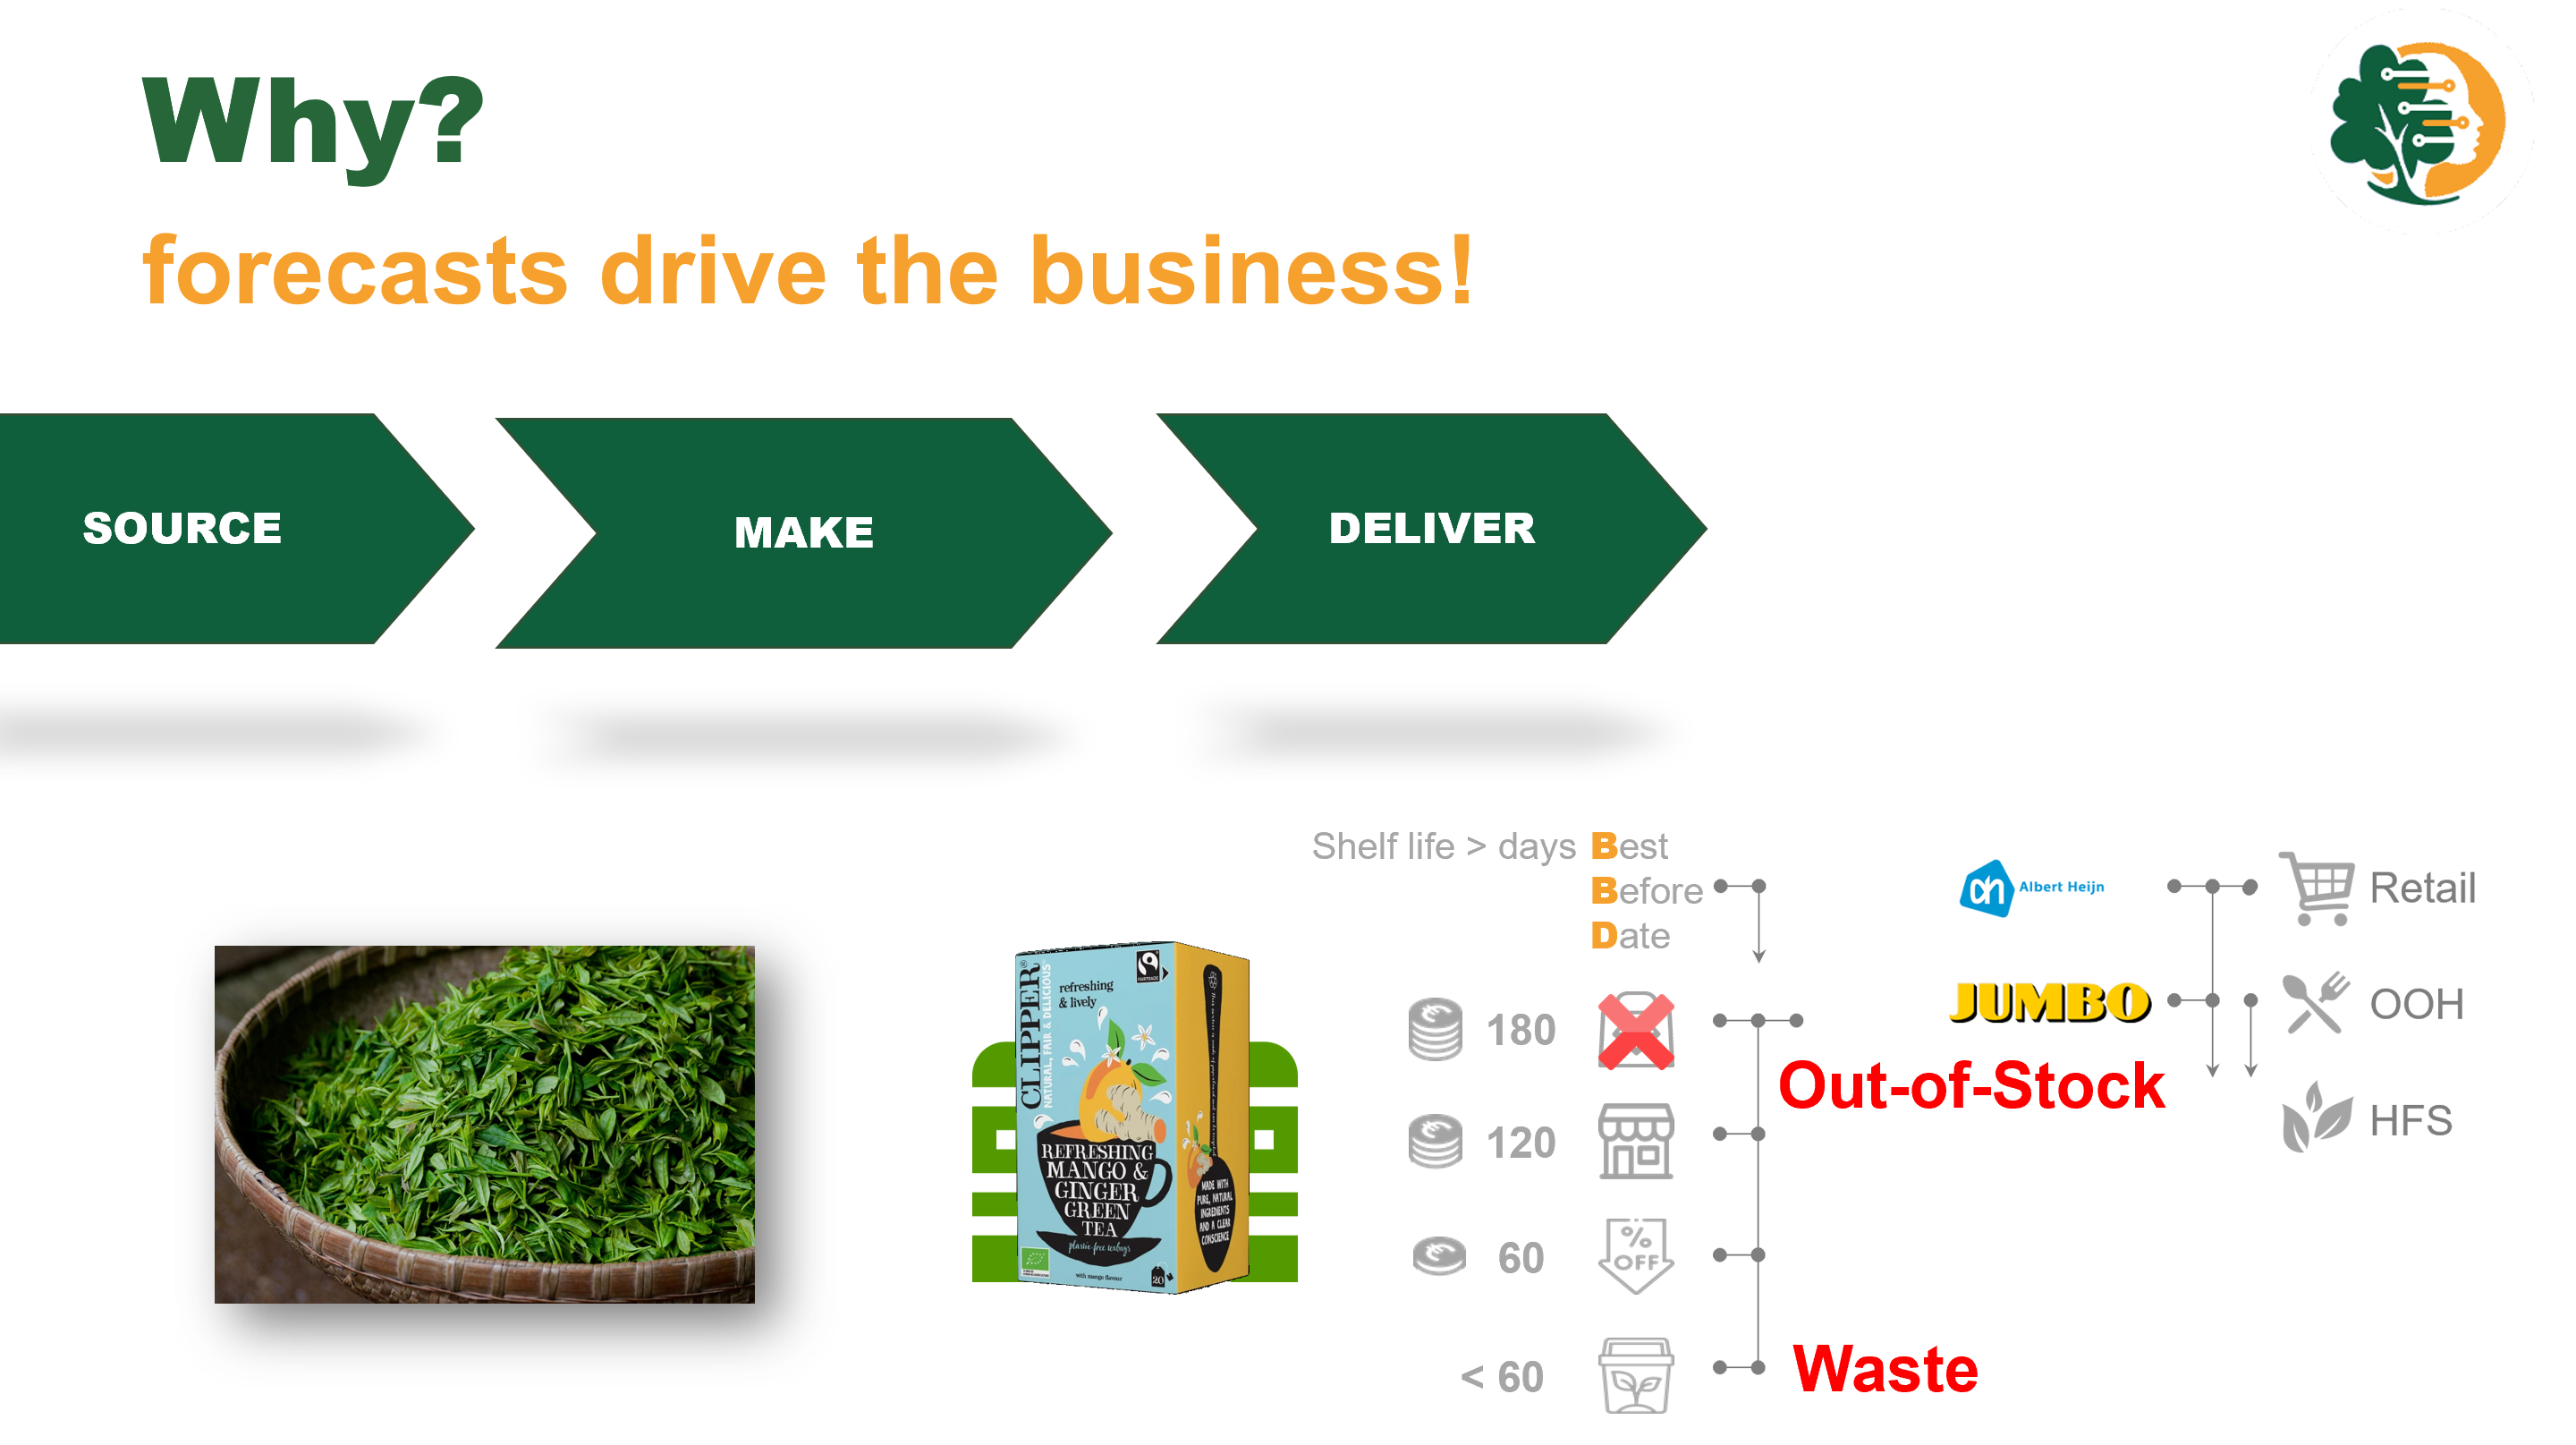
\includegraphics[keepaspectratio]{nb/../images/bu_why.png}}

\end{figure}%

See Figure Figure~\ref{fig-bu-why} for the thumbnail overview.

\chapter{Data Undestanding}\label{data-undestanding}

\chapter{Modeling}\label{modeling}

\chapter{Evaluation}\label{evaluation}

1.2\\
floris@smart-r.nl\\
\textbf{?meta:subtitle}

\begin{tcolorbox}[enhanced jigsaw, breakable, arc=.35mm, colbacktitle=quarto-callout-note-color!10!white, title=\textcolor{quarto-callout-note-color}{\faInfo}\hspace{0.5em}{Note}, colback=white, colframe=quarto-callout-note-color-frame, opacityback=0, bottomrule=.15mm, titlerule=0mm, leftrule=.75mm, left=2mm, rightrule=.15mm, bottomtitle=1mm, coltitle=black, toptitle=1mm, opacitybacktitle=0.6, toprule=.15mm]

Note that there are five types of callouts, including: \texttt{note},
\texttt{warning}, \texttt{important}, \texttt{tip}, and
\texttt{caution}.

\end{tcolorbox}

\begin{tcolorbox}[enhanced jigsaw, breakable, arc=.35mm, colbacktitle=quarto-callout-tip-color!10!white, title=\textcolor{quarto-callout-tip-color}{\faLightbulb}\hspace{0.5em}{Tip with Title}, colback=white, colframe=quarto-callout-tip-color-frame, opacityback=0, bottomrule=.15mm, titlerule=0mm, leftrule=.75mm, left=2mm, rightrule=.15mm, bottomtitle=1mm, coltitle=black, toptitle=1mm, opacitybacktitle=0.6, toprule=.15mm]

This is an example of a callout with a title.

\end{tcolorbox}

\begin{tcolorbox}[enhanced jigsaw, breakable, arc=.35mm, colbacktitle=quarto-callout-caution-color!10!white, title=\textcolor{quarto-callout-caution-color}{\faFire}\hspace{0.5em}{Expand To Learn About Collapse}, colback=white, colframe=quarto-callout-caution-color-frame, opacityback=0, bottomrule=.15mm, titlerule=0mm, leftrule=.75mm, left=2mm, rightrule=.15mm, bottomtitle=1mm, coltitle=black, toptitle=1mm, opacitybacktitle=0.6, toprule=.15mm]

This is an example of a `folded' caution callout that can be expanded by
the user. You can use \texttt{collapse="true"} to collapse it by default
or \texttt{collapse="false"} to make a collapsible callout that is
expanded by default.

\end{tcolorbox}

\chapter{Deployment}\label{deployment}

\chapter{Conclusion}\label{conclusion}

\chapter*{Glossary}\label{glossary}
\addcontentsline{toc}{chapter}{Glossary}

\markboth{Glossary}{Glossary}

\chapter{Conclusions}\label{conclusions}

Conclusions subtitle

\hfill\break

3\%

\part{Appendix}

\chapter{CRISP-DM}\label{crisp-dm}

\section{CRISP-DM}\label{sec-crisp-dm}

\begin{figure}[H]

\caption{Project Plan}

{\centering 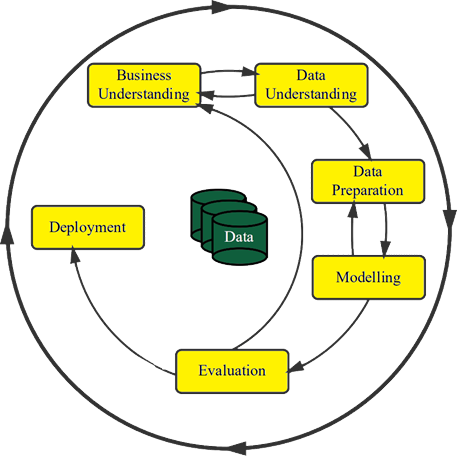
\includegraphics[width=0.7\linewidth,height=\textheight,keepaspectratio]{nb/../images/crisp-dm.png}

}

\end{figure}%

\chapter{Business Understanding}\label{business-understanding-1}

What is the business need?

\hfill\break

\begin{figure}

\caption{\label{fig-bu-why}Why forecasting?\\
The forecast drives the business!}

\pandocbounded{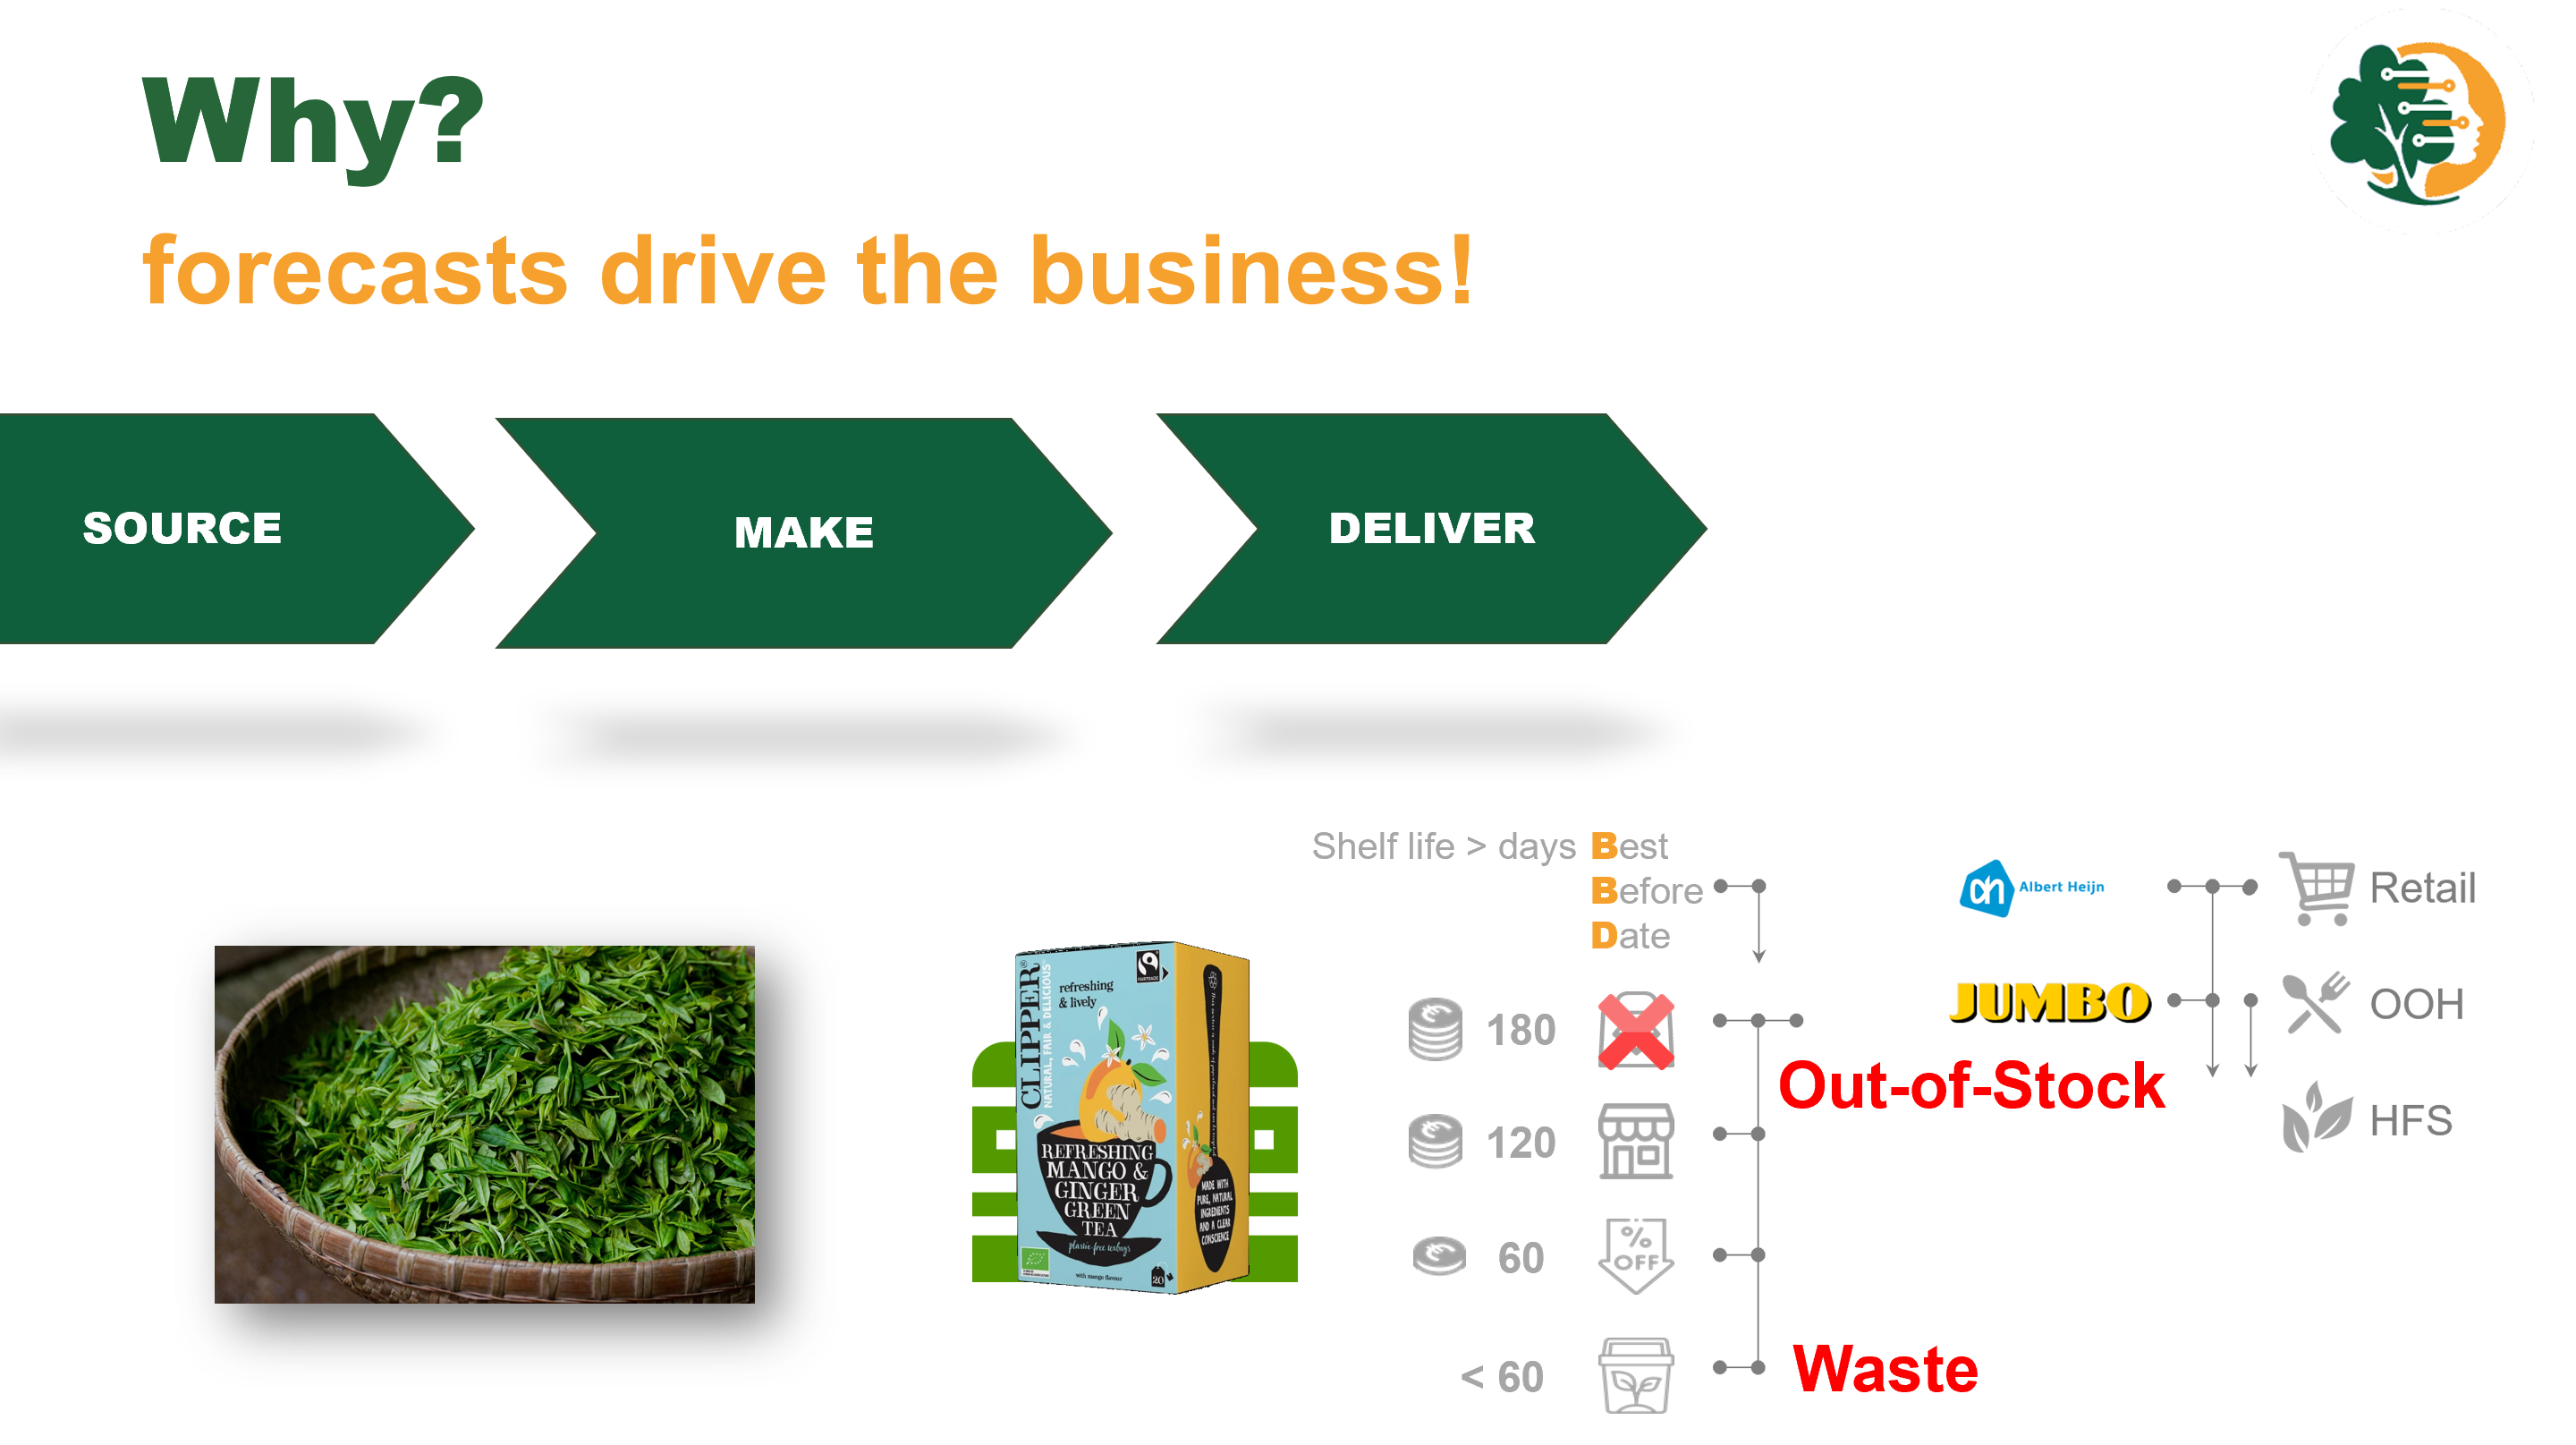
\includegraphics[keepaspectratio]{nb/../images/bu_why.png}}

\end{figure}%

See Figure Figure~\ref{fig-bu-why} for the thumbnail overview.

\section{Defining the Scope of the ML
Application}\label{defining-the-scope-of-the-ml-application}

\#\#Success Criteria - Business Success purpose and success criteria
(reduction OOS\&OOD) and other factors like customer \& employee
satisfaction - ML Success FA\% and BIAS\% - Economic Success impact of
the project on the companies financial performance DAPS \#\# Feasibility
availability, size, and quality of the training sample

\subsection{Background}\label{background}

The company's forecasting requirements vary significantly across several
key use cases, among others:

\begin{figure}[H]

\caption{supply chain network (sample)}

{\centering \pandocbounded{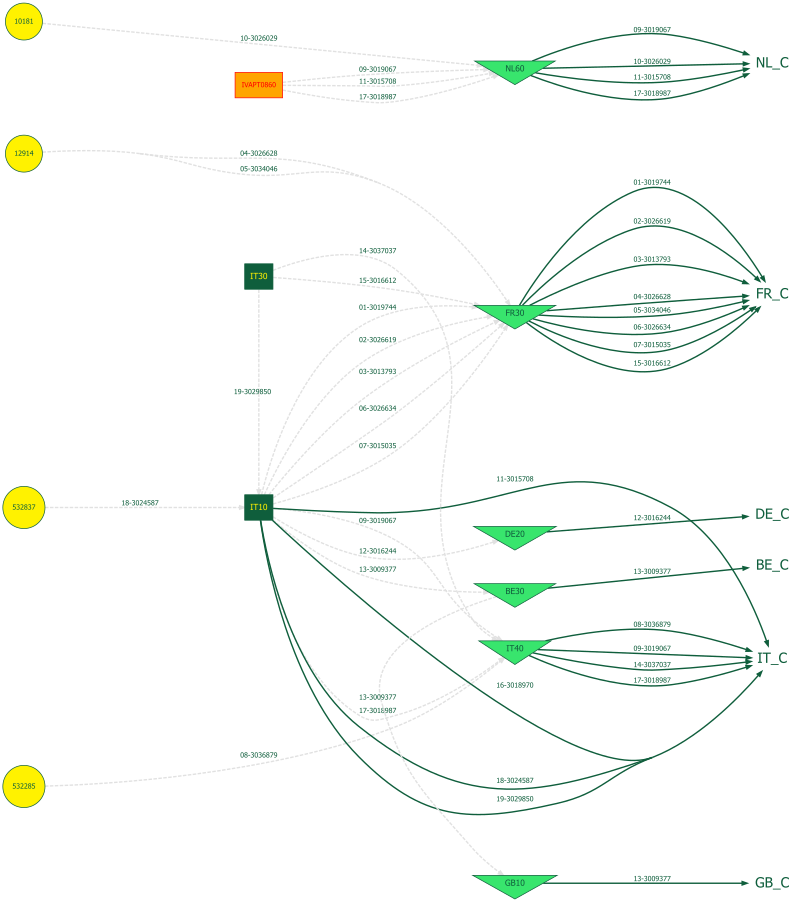
\includegraphics[keepaspectratio]{nb/../images/scn.png}}

}

\end{figure}%

\begin{enumerate}
\def\labelenumi{\arabic{enumi}.}
\item
  \textbf{Buying and Production}: Requires forecasts at the
  \textbf{material level} and \textbf{warehouse}, aggregated weekly,
  with a forecast horizon of \textbf{12 weeks}.
\item
  \textbf{Setting Safety Stock Profiles}: Requires forecasts at the
  \textbf{material level} and \textbf{warehouse}, aggregated weekly,
  with a forecast horizon of \textbf{26-52 weeks}, to determine safety
  stock profiles based on realized forecast accuracy.
\item
  \textbf{Negotiation with Customers}: Requires forecasts at a
  \textbf{monthly level}, aggregated by \textbf{material categories} and
  \textbf{customer groups}, with a horizon of \textbf{6 months}.
\item
  \textbf{Production Cost Calculation}: Requires forecasts at a
  \textbf{quarterly level}, aggregated by material, with a horizon of
  \textbf{6 quarters}, grouped into annual time buckets.
\end{enumerate}

The primary forecasting challenge is determining the optimal aggregation
level and methods to use for generating forecasts that can meet the
desired forecast accuracy of these different use cases while ensuring
\textbf{consistency} and \textbf{accuracy}.

This inconsistency stems from a lack of objective criteria for selecting
between forecasting methods---\textbf{bottom-up}, \textbf{top-down}, or
\textbf{middle-out}---resulting in decisions that rely on the subjective
judgment of demand planners, leading to variable performance and
inefficiencies.

\subsection{Business Objectives}\label{business-objectives}

The primary objective is to enhance operational efficiency by improving
forecast accuracy across all key use cases. This will be achieved
through the application of robust forecasting methods that can handle
seasonality, promotions, and efficiently allocate scarce resources.
Ultimately, these improvements will contribute to improved stock levels
and a higher level of customer satisfaction, both key strategic goals
for the company.

\subsection{Business Success Criteria}\label{business-success-criteria}

Success will be measured by the following criteria:

\begin{enumerate}
\def\labelenumi{\arabic{enumi}.}
\tightlist
\item
  \textbf{Improved Forecast Accuracy}:

  \begin{itemize}
  \tightlist
  \item
    \textbf{Tailored Forecasts for Each Use Case}: Enhanced accuracy
    across areas such as buying, production, safety stock settings, and
    customer negotiations, using methods that account for seasonality,
    promotions, and varying aggregation levels.
  \item
    \textbf{Reduced Forecast Errors and Bias}: Measurable reductions in
    key error metrics like RMSE , MAPE , and BIAS will lead to better
    alignment between forecasted and actual sales. Increased accuracy
    will also foster trust among supply planners, reducing the need for
    excessive safety margins.
  \item
    \textbf{Consistency Across Aggregation Levels}: Forecasts will
    remain consistent across different levels of aggregation, ensuring
    that detailed and aggregated forecasts are aligned.
  \end{itemize}
\item
  \textbf{Informed Decision-Making for Forecasting System
  Functionality}:

  \begin{itemize}
  \tightlist
  \item
    \textbf{Selecting the Right Forecasting Methods}: This research will
    guide the selection of optimal forecasting methods (statistical,
    machine learning, or hybrid) to improve performance across various
    use cases.
  \item
    \textbf{Efficient Resource Allocation}: A product classification
    scheme (e.g., ABC-XYZ) will be developed to help demand planners
    focus on high-impact products, while low-impact products will be
    managed more efficiently through automated forecasts.
  \end{itemize}
\item
  \textbf{Operational Benefits}:

  \begin{itemize}
  \tightlist
  \item
    \textbf{Improved Inventory Management}: More accurate forecasts will
    drive better purchasing and production decisions, leading to:

    \begin{itemize}
    \tightlist
    \item
      \textbf{Reduced Out-of-Stock (OOS) Incidents}: Ensuring product
      availability to meet customer demand and reduce penalties from
      stock-outs.
    \item
      \textbf{Reduced Out-of-Date (OOD) Incidents}: Minimizing waste and
      ensuring the freshness of perishable goods, leading to lower
      storage costs and better inventory turnover.
    \end{itemize}
  \item
    \textbf{Optimized Safety Stock Levels}: Accurate forecasts will
    allow for better safety stock settings, reducing both overstocking
    and stock-outs.
  \item
    \textbf{Cost Optimization}: Improved demand alignment will lower
    excess inventory and warehousing costs, minimize spoilage, and
    reduce costs associated with last-minute adjustments and
    overproduction.
  \end{itemize}
\item
  \textbf{Enhanced Supply Chain Efficiency and Decision-Making}:

  \begin{itemize}
  \tightlist
  \item
    \textbf{Strategic Decision Support}: Consistent and accurate
    forecasts will improve decision-making across production planning,
    sales target setting, capacity management, and workforce
    optimization. These improvements will also support better customer
    negotiations and more precise COGS (Cost of Goods Sold)
    calculations, resulting in a more efficient supply chain.
  \item
    \textbf{Increased Customer Satisfaction}: Improved product
    availability, fewer stock-outs, and fresher goods will not only
    reduce operational costs but will also enhance customer satisfaction
    and loyalty---a core strategic objective of the company.
  \end{itemize}
\end{enumerate}

By achieving these objectives, the company will see significant
improvements in operational efficiency, cost-effectiveness, and most
importantly, a higher level of customer satisfaction, which will
ultimately drive long-term business success.

see upper part of the flow-down graph, (Section~\ref{sec-flowdown}).

\subsection{Inventory of Resources
Requirements}\label{inventory-of-resources-requirements}

\subsubsection{Data sources:}\label{data-sources}

The available data includes \textbf{historical sales},
\textbf{promotional data}, \textbf{stock quantities}, and
\textbf{previous forecasts}. Stock-out periods will be adjusted for by
inflating sales to reflect demand that would have occurred had stock
been available.

\begin{longtable}[]{@{}
  >{\raggedright\arraybackslash}p{(\linewidth - 4\tabcolsep) * \real{0.3333}}
  >{\raggedright\arraybackslash}p{(\linewidth - 4\tabcolsep) * \real{0.3333}}
  >{\raggedright\arraybackslash}p{(\linewidth - 4\tabcolsep) * \real{0.3333}}@{}}
\toprule\noalign{}
\begin{minipage}[b]{\linewidth}\raggedright
Data Type
\end{minipage} & \begin{minipage}[b]{\linewidth}\raggedright
Details
\end{minipage} & \begin{minipage}[b]{\linewidth}\raggedright
Time Span
\end{minipage} \\
\midrule\noalign{}
\endhead
\bottomrule\noalign{}
\endlastfoot
Sales & Customer Orders, Inter-company, Returns, Free-of-Charge and
Missed & \textgreater{} 2020 \\
Promotions & Promotions per material and customer & \textgreater{}
2020 \\
Stock & Daily stock level per material and distribution center &
\textgreater{} 2020 \\
Forecasts & generated forecast before- and after Demand Review &
\textgreater{} Aug.~2023 \\
Master data & Material, Customer and Organization, including hierarchy's
& \emph{N.A.} \\
\end{longtable}

\subsubsection{Scoping}\label{scoping}

The scope of the project consist of two Marketing \& Sales Organizations
(MSO), with a focus on 6 brands, representing 5 out of the 6 categories,
see Table~\ref{tbl-material-scope}. These materials are made-to-stock
(MTS), requirements are planned on a weekly level, which represents 97\%
of the business.

This leaves us with about 1.000 materials out of 9.000 to focus on,
making the assumption that these are representative for the rest of the
products.

\begin{longtable}[]{@{}ll@{}}
\caption{Brands and Categories}\label{tbl-material-scope}\tabularnewline
\toprule\noalign{}
Brand & Category \\
\midrule\noalign{}
\endfirsthead
\toprule\noalign{}
Brand & Category \\
\midrule\noalign{}
\endhead
\bottomrule\noalign{}
\endlastfoot
Bjorg & Dairy \\
Clipper & Tea / Coffee \\
Naturela & Tea / Coffee \\
Tanoshi & Meals \\
Alter Eco & Sweets \\
Zonnatura & Breakfast Cereals \\
\end{longtable}

\subsection{Data Mining Goals}\label{data-mining-goals}

Predictive Model based on Correlations: Forecast Future Sales +
Promotion effects

see lower part of the flow-down graph, (Section~\ref{sec-flowdown}).

\subsubsection*{Data and Forecasting
Methods}\label{data-and-forecasting-methods}
\addcontentsline{toc}{subsubsection}{Data and Forecasting Methods}

We will employ a combination of \textbf{statistical methods} and
\textbf{machine learning techniques} to improve the forecasting process:

\begin{itemize}
\item
  \textbf{Current Methods}: The company's current forecasting system
  uses \textbf{moving averages}, \textbf{exponential smoothing} and
  \textbf{Box-Jenkins}, which face challenges with \textbf{Seasonality},
  \textbf{Stationarity} and \textbf{promotional effects}. Forecasts are
  often inadequate in handling the impacts of promotions.
\item
  \textbf{Proposed Methods}:

  \begin{itemize}
  \item
    \textbf{ETS (Error, Trend, Seasonal)}: To replace exponential
    smoothing with a model that provides \textbf{prediction intervals}
    and better captures trends and seasonality.
  \item
    \textbf{HTS (Hierarchical Time Series)}: To handle multiple
    aggregation levels, ensuring \textbf{forecast consistency} when
    forecasts are disaggregated or aggregated across levels.
  \item
    \textbf{XGBoost}: A machine learning technique capable of handling
    \textbf{promotional impacts} and even identifying
    \textbf{cannibalization effects} of promotions between products.
  \item
    \textbf{conformal prediction}: A method that provides
    \textbf{prediction intervals} and \textbf{calibrated forecasts},
    ensuring that the forecasted values are within a certain confidence
    level.
  \item
    \textbf{CatBoost and SHAP}: These will be used for feature analysis,
    determining which features (e.g., promotions, stock-outs) have the
    highest impact on forecast accuracy. This approach helps in choosing
    relevant input features to improve forecasts.
  \end{itemize}
\end{itemize}

\subsubsection*{Consistency and
Validation}\label{consistency-and-validation}
\addcontentsline{toc}{subsubsection}{Consistency and Validation}

One key requirement is ensuring that forecasts remain consistent across
different levels of aggregation. This is where \textbf{HTS} will play a
crucial role, reconciling forecasts generated at different aggregation
levels to ensure that top-level forecasts align with aggregated
lower-level forecasts. This will address the known issue of
discrepancies between aggregated forecasts and directly forecasted
aggregated levels.

\subsubsection{\texorpdfstring{\textbf{Human Resources
Allocation}}{Human Resources Allocation}}\label{human-resources-allocation}

The team consists of \textbf{X demand planners} working across \textbf{Y
MSOs}. Currently, planners are involved in manually indicating
promotional impacts and adjusting forecasts based on intuition, without
systematic data cleaning for stock-outs or model tuning.

To optimize resource allocation, we plan to implement a
\textbf{classification system} for the company's \textbf{9K SKUs},
utilizing an:

\textbf{ABC-XYZ classification} scheme:

\begin{itemize}
\tightlist
\item
  \textbf{ABC Classification}: Based on \textbf{sales volume}---focusing
  more resources on high-value items (A-class) and minimizing attention
  to low-volume items (C-class).
\item
  \textbf{XYZ Classification}: Based on \textbf{sales variability},
  indicating which products have stable demand versus those with erratic
  patterns.
\item
  \textbf{Combined Classification}: These classifications will guide
  planners in determining where their efforts can have the most impact,
  focusing primarily on high-priority items while relying more on
  automated processes for low-priority ones.
\end{itemize}

\subsection{Data Mining Success
Criteria}\label{data-mining-success-criteria}

The fiinal result will show an estimated relationship between forecast
accuracy and the cost of resources required for the agreed scope. The
cost of resources result from hardware, software and human resources
needed for cleansing data, transforming data, model tuning and other
manual activities needed.

To assess forecast accuracy, we will use a range of evaluation metrics
tailored to each use case.

These metrics will help evaluate how well each approach performs against
the unique requirements of each use case, ultimately guiding method
selection and refinement.

\begin{itemize}
\item
  \textbf{RMSE (Root Mean Squared Error, def~\ref{def-01-RMSE} )}: The
  primary metric for measuring forecast accuracy, particularly useful
  for penalizing large errors.
\item
  \textbf{MAPE (Mean Absolute Percentage Error)}: To align with existing
  company metrics.
\item
  \textbf{MAE (Mean Absolute Error)} and \textbf{MASE (Mean Absolute
  Scaled Error)}: Additional metrics to provide a broader evaluation,
  addressing different aspects of forecast performance and comparing
  models to naïve baselines.
\end{itemize}

\subsection{Project Plan}\label{project-plan}

see Section~\ref{sec-project-plan}

\subsubsection{Initial Assessment of Tools and
Techniques}\label{initial-assessment-of-tools-and-techniques}

see Literature review (Section~\ref{sec-literature_review})

\begin{definition}[]\protect\hypertarget{def-01-RMSE}{}\label{def-01-RMSE}

\textbf{RMSE:}

Root Mean Squared Error

RMSE = \(\sqrt{mean(e^2_t)}\)

A
\href{https://otexts.com/fpp3/accuracy.html\#scale-dependent-errors}{Scale-dependent
error}, to compare forecast performances between data sets with the same
unit.

\end{definition}

\chapter{Data Understanding}\label{data-understanding}

Data Understanding subtitle

\hfill\break

\section{Data Collection Report}\label{data-collection-report}

\section{Data Description Report}\label{data-description-report}

\section{Data Exploration Report}\label{data-exploration-report}

\section{Data Quality Report}\label{data-quality-report}

\section{Identification of Data
Sources}\label{identification-of-data-sources}

\section{Data Quality Assessment}\label{data-quality-assessment}

assessing the - completeness: impute missing data - accuracy: =
consistency:

\subsection{Data Description}\label{data-description}

A descriptive exploratory analysis describes the data by its statistical
properties and metadata.

outliers?

\subsection{Data Verification}\label{data-verification}

\chapter{Data Preparation}\label{data-preparation}

preparing the data for further analysis and modeling. This might involve
cleaning and preprocessing the data, as well as transforming it into a
format that is suitable for use in a machine-learning model.

5.1. Handling Missing Data

\begin{itemize}
\item
  imputing missing values, Imputation methods involve replacing missing
  values with estimated values.
\item
  scaling numeric features
\item
  encoding categorical features
\item
  selecting a subset of the data to use in the model.
\end{itemize}

\begin{figure}

\caption{\label{fig-plot-penguins}Bill length vs.~depth for Palmer
Penguins}

\centering{

\pandocbounded{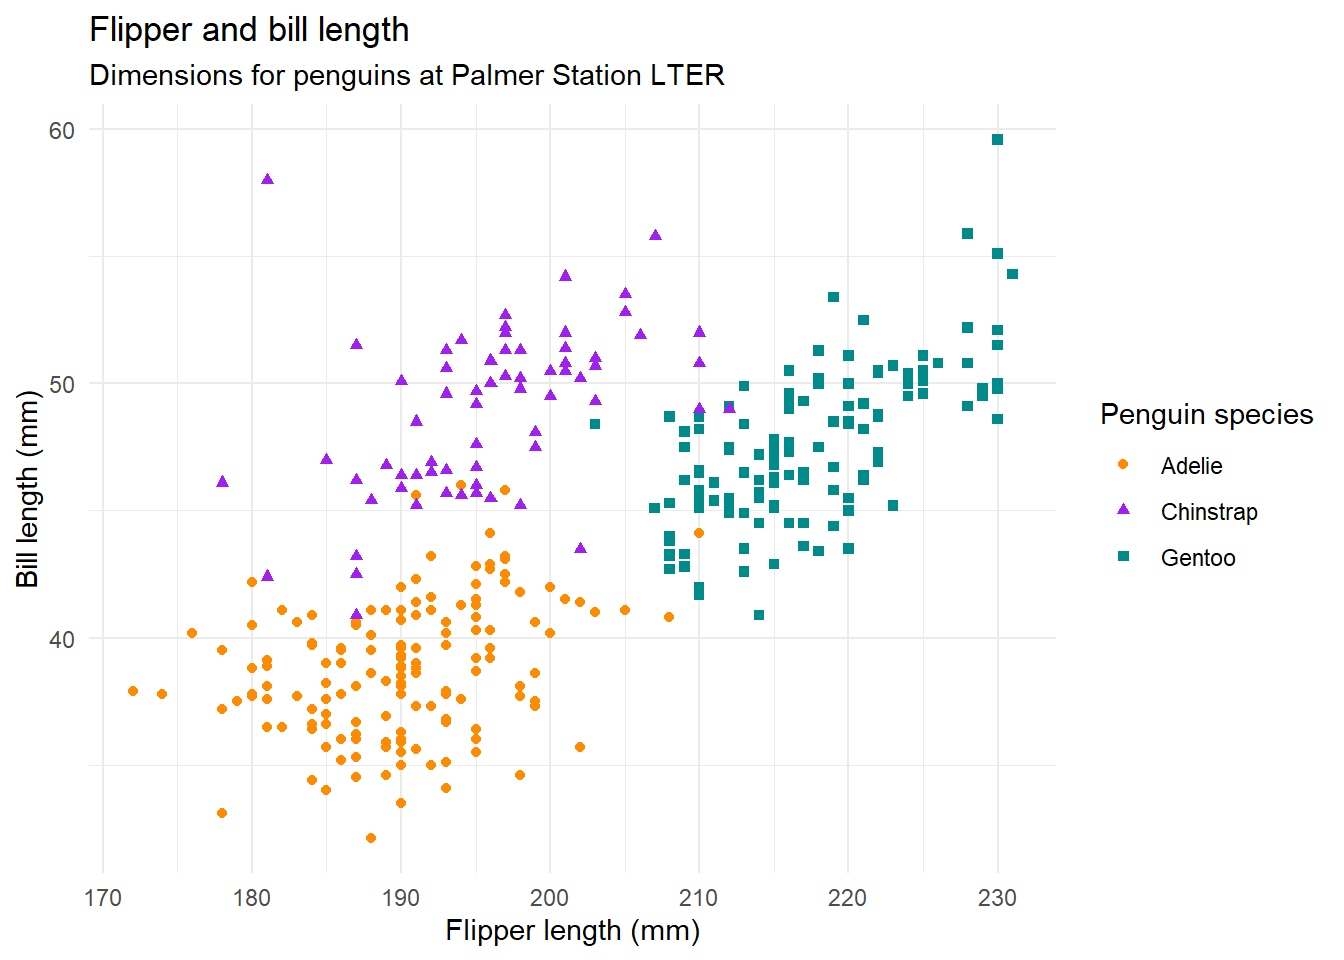
\includegraphics[keepaspectratio]{nb/02_data_understanding_rev_files/figure-pdf/fig-plot-penguins-1.pdf}}

}

\end{figure}%

\begin{verbatim}
          uid               text   cnt
       <char>             <char> <int>
 1:         1        Electronics    11
 2:       1.4          Computers    11
 3:    1.4.10            Laptops    11
 4: 1.4.10.20         Ultrabooks    11
 5:    1.4.11           Desktops    11
 6: 1.4.11.21             Gaming    11
 7:    1.4.12            Tablets    11
 8: 1.4.12.22              iPads    11
 9:       1.5                TVs    11
10:    1.5.13                LED    11
11: 1.5.13.23            Samsung    11
12:         2               Home     9
13:       2.6            Kitchen     9
14:    2.6.14         Appliances     9
15: 2.6.14.24              Ovens     9
16:    2.6.15           Cookware     9
17: 2.6.15.25               Pots     9
18:       2.7          Furniture     9
19:    2.7.16             Chairs     9
20: 2.7.16.26       OfficeChairs     9
21:         3             Garden     9
22:       3.8             Plants     9
23:    3.8.17            Flowers     9
24: 3.8.17.27              Roses     9
25:    3.8.18              Trees     9
26: 3.8.18.28               Oaks     9
27:       3.9              Tools     9
28:    3.9.19         PowerTools     9
29: 3.9.19.29             Drills     9
          uid               text   cnt
\end{verbatim}

\begin{Shaded}
\begin{Highlighting}[]
\FunctionTok{library}\NormalTok{(ggplot2)}
\FunctionTok{library}\NormalTok{(data.table)}
\FunctionTok{library}\NormalTok{(lubridate)}
\FunctionTok{library}\NormalTok{(magrittr)}
\FunctionTok{library}\NormalTok{(stringr)}
\FunctionTok{library}\NormalTok{(openxlsx)}

\FunctionTok{library}\NormalTok{(tidyverse)}

\NormalTok{LP0 }\OtherTok{\textless{}{-}} 
  \ControlFlowTok{function}\NormalTok{(x, width)\{}
    \CommentTok{\# like CONVERSION\_EXIT\_MATN1\_INPUT}
    \CommentTok{\# only add leading zero\textquotesingle{}s in case it is a number}
\NormalTok{    is\_num }\OtherTok{\textless{}{-}} \FunctionTok{grepl}\NormalTok{(}\StringTok{"\^{}[0{-}9]+$"}\NormalTok{, x)}
    \FunctionTok{ifelse}\NormalTok{(}
\NormalTok{      is\_num, }
\NormalTok{      stringr}\SpecialCharTok{::}\FunctionTok{str\_pad}\NormalTok{(}\AttributeTok{string =}\NormalTok{ x, }\AttributeTok{width =}\NormalTok{ width, }\AttributeTok{side =} \StringTok{"left"}\NormalTok{, }\AttributeTok{pad =} \StringTok{"0"}\NormalTok{),}
\NormalTok{      x}
\NormalTok{    )}
\NormalTok{  \}}

\NormalTok{fOpen\_as\_xlsx }\OtherTok{\textless{}{-}} 
  \ControlFlowTok{function}\NormalTok{(pDT, }\AttributeTok{pPath =} \StringTok{"./Results"}\NormalTok{, pFN, }\AttributeTok{pasTable =} \ConstantTok{TRUE}\NormalTok{)\{}
    
    \ControlFlowTok{if}\NormalTok{ (}\SpecialCharTok{!}\FunctionTok{dir.exists}\NormalTok{(pPath)) \{}
      \FunctionTok{dir.create}\NormalTok{(pPath)}
\NormalTok{    \}}
    
    \ControlFlowTok{if}\NormalTok{ (}\FunctionTok{missing}\NormalTok{(pFN) }\SpecialCharTok{==} \ConstantTok{TRUE}\NormalTok{) \{}
\NormalTok{      pFN }\OtherTok{\textless{}{-}} \FunctionTok{paste0}\NormalTok{(}\StringTok{"\textasciitilde{}"}\NormalTok{, }\FunctionTok{format}\NormalTok{(}\FunctionTok{now}\NormalTok{(), }\StringTok{"\%Y\%m\%d{-}\%H\%M\%S"}\NormalTok{), }\StringTok{".xlsx"}\NormalTok{)}
\NormalTok{    \}}
    
\NormalTok{    FFN }\OtherTok{\textless{}{-}} \FunctionTok{file.path}\NormalTok{(pPath, pFN)}
    \FunctionTok{write.xlsx}\NormalTok{(}\AttributeTok{x =}\NormalTok{ pDT, }\AttributeTok{file =}\NormalTok{ FFN, }\AttributeTok{asTable =}\NormalTok{ pasTable, }\AttributeTok{tableStyle =} \StringTok{"TableStyleMedium4"}\NormalTok{) }
    \FunctionTok{openXL}\NormalTok{(FFN)}
    
\NormalTok{  \}}
\CommentTok{\# PDAT \textless{}{-} file.path("C:", "PW", "OneDrive", "ET", "pythia", "dat")}

\NormalTok{PDAT }\OtherTok{\textless{}{-}} 
  \ControlFlowTok{switch}\NormalTok{(}\FunctionTok{Sys.info}\NormalTok{()[}\StringTok{"nodename"}\NormalTok{],}
         \StringTok{\textquotesingle{}TREX{-}TOAD\textquotesingle{}} \OtherTok{=} \FunctionTok{file.path}\NormalTok{(}\StringTok{"U:"}\NormalTok{, }\StringTok{"floris"}\NormalTok{),}
                       \FunctionTok{file.path}\NormalTok{(}\StringTok{"C:"}\NormalTok{, }\StringTok{"PW"}\NormalTok{)}
\NormalTok{  ) }\SpecialCharTok{\%\textgreater{}\%} 
  \FunctionTok{file.path}\NormalTok{(}\StringTok{"OneDrive"}\NormalTok{, }\StringTok{"ET"}\NormalTok{, }\StringTok{"pythia"}\NormalTok{, }\StringTok{"dat"}\NormalTok{)}

\NormalTok{ET\_CG }\OtherTok{\textless{}{-}} \StringTok{"\#0f5e3c"}
\NormalTok{ET\_FG }\OtherTok{\textless{}{-}} \StringTok{"\#089b35"}

\NormalTok{MAT }\OtherTok{\textless{}{-}} \StringTok{\textquotesingle{}000000000003036397\textquotesingle{}}
\NormalTok{MAN }\OtherTok{\textless{}{-}} \ConstantTok{FALSE} \SpecialCharTok{\&} \FunctionTok{substr}\NormalTok{(PDAT, }\DecValTok{1}\NormalTok{,}\DecValTok{1}\NormalTok{) }\SpecialCharTok{!=} \StringTok{"U"}

\NormalTok{BRNDS }\OtherTok{\textless{}{-}} 
  \FunctionTok{fread}\NormalTok{(}\AttributeTok{text =} \StringTok{"}
\StringTok{  PRDH1, NAME}
\StringTok{  07   , ALTER ECO}
\StringTok{  08   , BJORG}
\StringTok{  10   , CLIPPER (CUPPER)}
\StringTok{  15   , ZONNATURA}
\StringTok{  53   , TANOSHI}
\StringTok{  65   , NATURELA"}
\NormalTok{  ) }\SpecialCharTok{\%\textgreater{}\%}
\NormalTok{  .[, PRDH1}\SpecialCharTok{:}\ErrorTok{=} \FunctionTok{str\_pad}\NormalTok{(PRDH1, }\DecValTok{2}\NormalTok{, }\AttributeTok{pad =} \StringTok{"0"}\NormalTok{)]}
\end{Highlighting}
\end{Shaded}

\section{SDMFRCAC FA}\label{sdmfrcac-fa}

\begin{Shaded}
\begin{Highlighting}[]
\NormalTok{B4\_SDMFRCAC2\_A }\OtherTok{\textless{}{-}} 
  \FunctionTok{readRDS}\NormalTok{(}\AttributeTok{file =} \FunctionTok{file.path}\NormalTok{(PDAT, }\StringTok{"B4\_SDMFRCAC2\_A.rds"}\NormalTok{))              }\SpecialCharTok{\%\textgreater{}\%}
\NormalTok{  .[PLANT }\SpecialCharTok{\%chin\%} \FunctionTok{c}\NormalTok{(}\StringTok{"FR30"}\NormalTok{, }\StringTok{"NL60"}\NormalTok{, }\StringTok{"NL63"}\NormalTok{)]}

\NormalTok{B4\_MATERIAL\_P  }\OtherTok{\textless{}{-}} 
  \FunctionTok{readRDS}\NormalTok{(}\AttributeTok{file =} \FunctionTok{file.path}\NormalTok{(PDAT, }\StringTok{"B4\_MATERIAL\_P.rds"}\NormalTok{))               }\SpecialCharTok{\%\textgreater{}\%}
\NormalTok{  .[MATL\_TYPE }\SpecialCharTok{\%chin\%} \FunctionTok{c}\NormalTok{(}\StringTok{"FERT"}\NormalTok{, }\StringTok{"HALB"}\NormalTok{)]}

\NormalTok{dtFA }\OtherTok{\textless{}{-}} 
\NormalTok{  BRNDS[B4\_MATERIAL\_P[MATL\_TYPE }\SpecialCharTok{\%chin\%} \FunctionTok{c}\NormalTok{(}\StringTok{"FERT"}\NormalTok{, }\StringTok{"HALB"}\NormalTok{)], }
\NormalTok{        on }\OtherTok{=}\NormalTok{ .(}\AttributeTok{PRDH1 =}\NormalTok{ PRDH1), nomatch }\OtherTok{=} \DecValTok{0}\NormalTok{]                          }\SpecialCharTok{\%\textgreater{}\%}
\NormalTok{  .[B4\_SDMFRCAC2\_A, on }\OtherTok{=}\NormalTok{ .(SYSTID, CLIENT, MATERIAL), nomatch }\OtherTok{=} \DecValTok{0}\NormalTok{]   }\SpecialCharTok{\%\textgreater{}\%}
\NormalTok{  .[, .(}
    \AttributeTok{ACT =} \FunctionTok{sum}\NormalTok{(DEMND\_QTY),}
    \AttributeTok{FM1 =} \FunctionTok{sum}\NormalTok{(DEMQTYM1)}
\NormalTok{  ), by }\OtherTok{=}\NormalTok{ .(PRDH1, PLANT, MATERIAL, CALMONTH)}
\NormalTok{  ]                                                                  }\SpecialCharTok{\%\textgreater{}\%}
\NormalTok{  .[, \{}
\NormalTok{    E   }\OtherTok{=}\NormalTok{ ACT }\SpecialCharTok{{-}}\NormalTok{ FM1}
\NormalTok{    E2  }\OtherTok{=}\NormalTok{ E }\SpecialCharTok{\^{}} \DecValTok{2}
\NormalTok{    AE  }\OtherTok{=} \FunctionTok{abs}\NormalTok{(E)}
\NormalTok{    APE }\OtherTok{=} \DecValTok{100} \SpecialCharTok{*}\NormalTok{ (}\DecValTok{1} \SpecialCharTok{{-}}\NormalTok{ AE }\SpecialCharTok{/}\NormalTok{ ACT)}
\NormalTok{    ECO }\OtherTok{=} \DecValTok{100} \SpecialCharTok{*}\NormalTok{ (}\DecValTok{1} \SpecialCharTok{{-}}\NormalTok{ AE }\SpecialCharTok{/}\NormalTok{ FM1)}
\NormalTok{    .(}
\NormalTok{      PRDH1, PLANT, MATERIAL, CALMONTH, }
\NormalTok{      ACT  , FM1  , E, E2, AE, APE, ECO}
\NormalTok{      )}
\NormalTok{  \}  ] }

\NormalTok{dtFA }\OtherTok{\textless{}{-}} 
\NormalTok{  dtFA[}
    \SpecialCharTok{!}\FunctionTok{is.nan}\NormalTok{(APE) }\SpecialCharTok{\&} 
    \SpecialCharTok{!}\FunctionTok{is.nan}\NormalTok{(ECO) }\SpecialCharTok{\&}   
    \SpecialCharTok{!}\FunctionTok{is.infinite}\NormalTok{(APE) }\SpecialCharTok{\&}
    \SpecialCharTok{!}\FunctionTok{is.infinite}\NormalTok{(ECO) }\SpecialCharTok{\&}  
\NormalTok{    APE }\SpecialCharTok{\textgreater{}} \SpecialCharTok{{-}}\DecValTok{100} \SpecialCharTok{\&}
\NormalTok{    ECO }\SpecialCharTok{\textgreater{}} \SpecialCharTok{{-}}\DecValTok{100}\NormalTok{  ]}
\end{Highlighting}
\end{Shaded}

\begin{Shaded}
\begin{Highlighting}[]
\NormalTok{PYT }\OtherTok{\textless{}{-}} \FunctionTok{file.path}\NormalTok{(}\StringTok{"C:"}\NormalTok{, }\StringTok{"PW"}\NormalTok{, }\StringTok{"OneDrive"}\NormalTok{, }\StringTok{"ET"}\NormalTok{, }\StringTok{"pythia"}\NormalTok{, }\StringTok{"upg"}\NormalTok{, }\StringTok{"data"}\NormalTok{)}

\NormalTok{MATS }\OtherTok{\textless{}{-}} 
  \FunctionTok{fread}\NormalTok{(}\FunctionTok{file.path}\NormalTok{(PYT, }\StringTok{"MD\_MATERIAL\_SALES\_ORG.CSV"}\NormalTok{)) }\SpecialCharTok{\%\textgreater{}\%}
\NormalTok{  .[, MATERIAL }\SpecialCharTok{:}\ErrorTok{=} \FunctionTok{LP0}\NormalTok{(V1, }\DecValTok{18}\NormalTok{)] }

\NormalTok{TST }\OtherTok{\textless{}{-}} 
\NormalTok{  MATS[V2 }\SpecialCharTok{==} \StringTok{\textquotesingle{}NL10\textquotesingle{}}\NormalTok{, .(MATERIAL, }\AttributeTok{PLANT =} \StringTok{\textquotesingle{}NL60\textquotesingle{}}\NormalTok{, }\AttributeTok{PROMO =}\NormalTok{ V17)][}
\NormalTok{    B4\_SDMFRCAC2\_A, on }\OtherTok{=}\NormalTok{ .(MATERIAL, PLANT), nomatch }\OtherTok{=} \ConstantTok{NA}\NormalTok{] }\SpecialCharTok{\%\textgreater{}\%}
\NormalTok{  .[PLANT }\SpecialCharTok{!=} \StringTok{\textquotesingle{}FR30\textquotesingle{}}\NormalTok{]}
\end{Highlighting}
\end{Shaded}

\begin{Shaded}
\begin{Highlighting}[]
\NormalTok{MAT }\OtherTok{\textless{}{-}} \FunctionTok{LP0}\NormalTok{(}\StringTok{\textquotesingle{}10023\textquotesingle{}}\NormalTok{, }\DecValTok{18}\NormalTok{)}

\FunctionTok{ggplot}\NormalTok{(}
  \AttributeTok{data =}\NormalTok{ dtFA[}
\NormalTok{    MATERIAL }\SpecialCharTok{==}\NormalTok{ MAT}
\NormalTok{    ], }\FunctionTok{aes}\NormalTok{(}\AttributeTok{x =}\NormalTok{ CALMONTH, }\AttributeTok{y =}\NormalTok{ ACT)) }\SpecialCharTok{+}
  \FunctionTok{geom\_col}\NormalTok{(}\AttributeTok{fill =}\NormalTok{ ET\_CG) }\SpecialCharTok{+}
  \FunctionTok{theme\_minimal}\NormalTok{()}
\end{Highlighting}
\end{Shaded}

\begin{Shaded}
\begin{Highlighting}[]
\FunctionTok{ggplot}\NormalTok{(}
  \AttributeTok{data =}\NormalTok{ dtFA[}
\NormalTok{    CALMONTH }\SpecialCharTok{\textgreater{}=}\StringTok{\textquotesingle{}202401\textquotesingle{}} 
    \SpecialCharTok{\&}\NormalTok{ APE }\SpecialCharTok{\textgreater{}} \SpecialCharTok{{-}}\DecValTok{50}
    \CommentTok{\# \& MATERIAL == MAT}
\NormalTok{  ], }
  \FunctionTok{aes}\NormalTok{(}\AttributeTok{x =}\NormalTok{ APE, }\AttributeTok{y =}\NormalTok{ ECO)}
\NormalTok{) }\SpecialCharTok{+}
  \FunctionTok{geom\_point}\NormalTok{() }\SpecialCharTok{+}
  \FunctionTok{geom\_abline}\NormalTok{(}\AttributeTok{intercept =} \DecValTok{0}\NormalTok{, }\AttributeTok{slope =} \DecValTok{1}\NormalTok{) }\SpecialCharTok{+}
  \CommentTok{\# geom\_label(aes(label = round(PE, 1))) +}
  \CommentTok{\# facet\_wrap(\textasciitilde{} PLANT + MATERIAL, scales = "free\_y") +}
  \CommentTok{\# scale\_color\_manual(values=c(ET\_CG, ET\_FG))+}
  \FunctionTok{theme\_minimal}\NormalTok{()}
\end{Highlighting}
\end{Shaded}

\begin{Shaded}
\begin{Highlighting}[]
\NormalTok{dtFA\_melt  }\OtherTok{\textless{}{-}} 
  \FunctionTok{copy}\NormalTok{(dtFA) }\SpecialCharTok{\%\textgreater{}\%}
  \FunctionTok{melt.data.table}\NormalTok{(}
    \AttributeTok{measure.vars  =} \FunctionTok{c}\NormalTok{(}\StringTok{"APE"}\NormalTok{, }\StringTok{"ECO"}\NormalTok{),}
    \AttributeTok{variable.name =} \StringTok{"PE\_TYPE"}\NormalTok{,}
    \AttributeTok{value.name    =} \StringTok{"PE"}
\NormalTok{    ) }\SpecialCharTok{\%T\textgreater{}\%} \FunctionTok{setorder}\NormalTok{(CALMONTH)}

\FunctionTok{ggplot}\NormalTok{(}
  \AttributeTok{data =}\NormalTok{ dtFA\_melt[CALMONTH }\SpecialCharTok{\textgreater{}=}\StringTok{\textquotesingle{}202401\textquotesingle{}} \SpecialCharTok{\&}\NormalTok{ MATERIAL }\SpecialCharTok{==}\NormalTok{ MAT], }
  \FunctionTok{aes}\NormalTok{(}\AttributeTok{x =}\NormalTok{ CALMONTH, }\AttributeTok{y =}\NormalTok{ PE, }\AttributeTok{group =}\NormalTok{ PE\_TYPE, }\AttributeTok{color =}\NormalTok{ PE\_TYPE)}
\NormalTok{  ) }\SpecialCharTok{+}
  \FunctionTok{geom\_line}\NormalTok{(}\AttributeTok{linewidth =} \DecValTok{2}\NormalTok{) }\SpecialCharTok{+}
  \FunctionTok{geom\_point}\NormalTok{() }\SpecialCharTok{+}
  \FunctionTok{geom\_label}\NormalTok{(}\FunctionTok{aes}\NormalTok{(}\AttributeTok{label =} \FunctionTok{round}\NormalTok{(PE, }\DecValTok{1}\NormalTok{))) }\SpecialCharTok{+}
  \CommentTok{\# facet\_wrap(\textasciitilde{} PLANT + MATERIAL, scales = "free\_y") +}
  \FunctionTok{scale\_color\_manual}\NormalTok{(}\AttributeTok{values=}\FunctionTok{c}\NormalTok{(ET\_CG, ET\_FG))}\SpecialCharTok{+}
  \FunctionTok{theme\_minimal}\NormalTok{()}

\CommentTok{\# if(MAN)\{}
\CommentTok{\#   if(rstudioapi::showQuestion(}
\CommentTok{\#     title   = "SAC", }
\CommentTok{\#     message = "Do you want to open SC{-}113B?"}
\CommentTok{\#   ) == TRUE) \{}
\CommentTok{\#     browseURL(url = "https://wessanen.eu10.sapanalytics.cloud/link/SC113B")}
\CommentTok{\#   \}}
\CommentTok{\# \}}
\end{Highlighting}
\end{Shaded}

\begin{Shaded}
\begin{Highlighting}[]
\NormalTok{dtFA\_melt  }\OtherTok{\textless{}{-}} 
  \FunctionTok{copy}\NormalTok{(dtFA) }\SpecialCharTok{\%\textgreater{}\%}
  \FunctionTok{melt.data.table}\NormalTok{(}
    \AttributeTok{measure.vars  =} \FunctionTok{c}\NormalTok{(}\StringTok{"APE"}\NormalTok{, }\StringTok{"ECO"}\NormalTok{),}
    \AttributeTok{variable.name =} \StringTok{"PE\_TYPE"}\NormalTok{,}
    \AttributeTok{value.name    =} \StringTok{"PE"}
\NormalTok{    )                                         }\SpecialCharTok{\%T\textgreater{}\%} 
  \FunctionTok{setorder}\NormalTok{(PLANT, MATERIAL, CALMONTH)}

\FunctionTok{ggplot}\NormalTok{(}
  \AttributeTok{data =}\NormalTok{ dtFA\_melt[CALMONTH }\SpecialCharTok{\textgreater{}=}\StringTok{\textquotesingle{}202401\textquotesingle{}} \SpecialCharTok{\&}\NormalTok{ MATERIAL }\SpecialCharTok{==}\NormalTok{ MAT], }
  \FunctionTok{aes}\NormalTok{(}\AttributeTok{x =}\NormalTok{ CALMONTH, }\AttributeTok{y =}\NormalTok{ PE, }\AttributeTok{group =}\NormalTok{ PE\_TYPE, }\AttributeTok{color =}\NormalTok{ PE\_TYPE)}
\NormalTok{  ) }\SpecialCharTok{+}
  \FunctionTok{geom\_line}\NormalTok{(}\AttributeTok{linewidth =} \DecValTok{2}\NormalTok{) }\SpecialCharTok{+}
  \FunctionTok{geom\_point}\NormalTok{() }\SpecialCharTok{+}
  \FunctionTok{geom\_label}\NormalTok{(}\FunctionTok{aes}\NormalTok{(}\AttributeTok{label =} \FunctionTok{round}\NormalTok{(PE, }\DecValTok{1}\NormalTok{))) }\SpecialCharTok{+}
  \CommentTok{\# facet\_wrap(\textasciitilde{} PLANT + MATERIAL, scales = "free\_y") +}
  \FunctionTok{scale\_color\_manual}\NormalTok{(}\AttributeTok{values=}\FunctionTok{c}\NormalTok{(ET\_CG, ET\_FG))}\SpecialCharTok{+}
  \FunctionTok{theme\_minimal}\NormalTok{()}

\CommentTok{\# if(MAN)\{}
\CommentTok{\#   if(rstudioapi::showQuestion(}
\CommentTok{\#     title   = "SAC", }
\CommentTok{\#     message = "Do you want to open SC{-}113B?"}
\CommentTok{\#   ) == TRUE) \{}
\CommentTok{\#     browseURL(url = "https://wessanen.eu10.sapanalytics.cloud/link/SC113B")}
\CommentTok{\#   \}}
\CommentTok{\# \}}
\end{Highlighting}
\end{Shaded}

\chapter{Data Preparation}\label{data-preparation-1}

Data Preparation subtitle

\hfill\break

\begin{figure}

\caption{\label{fig-bu-why}Why forecasting?\\
The forecast drives the business!}

\pandocbounded{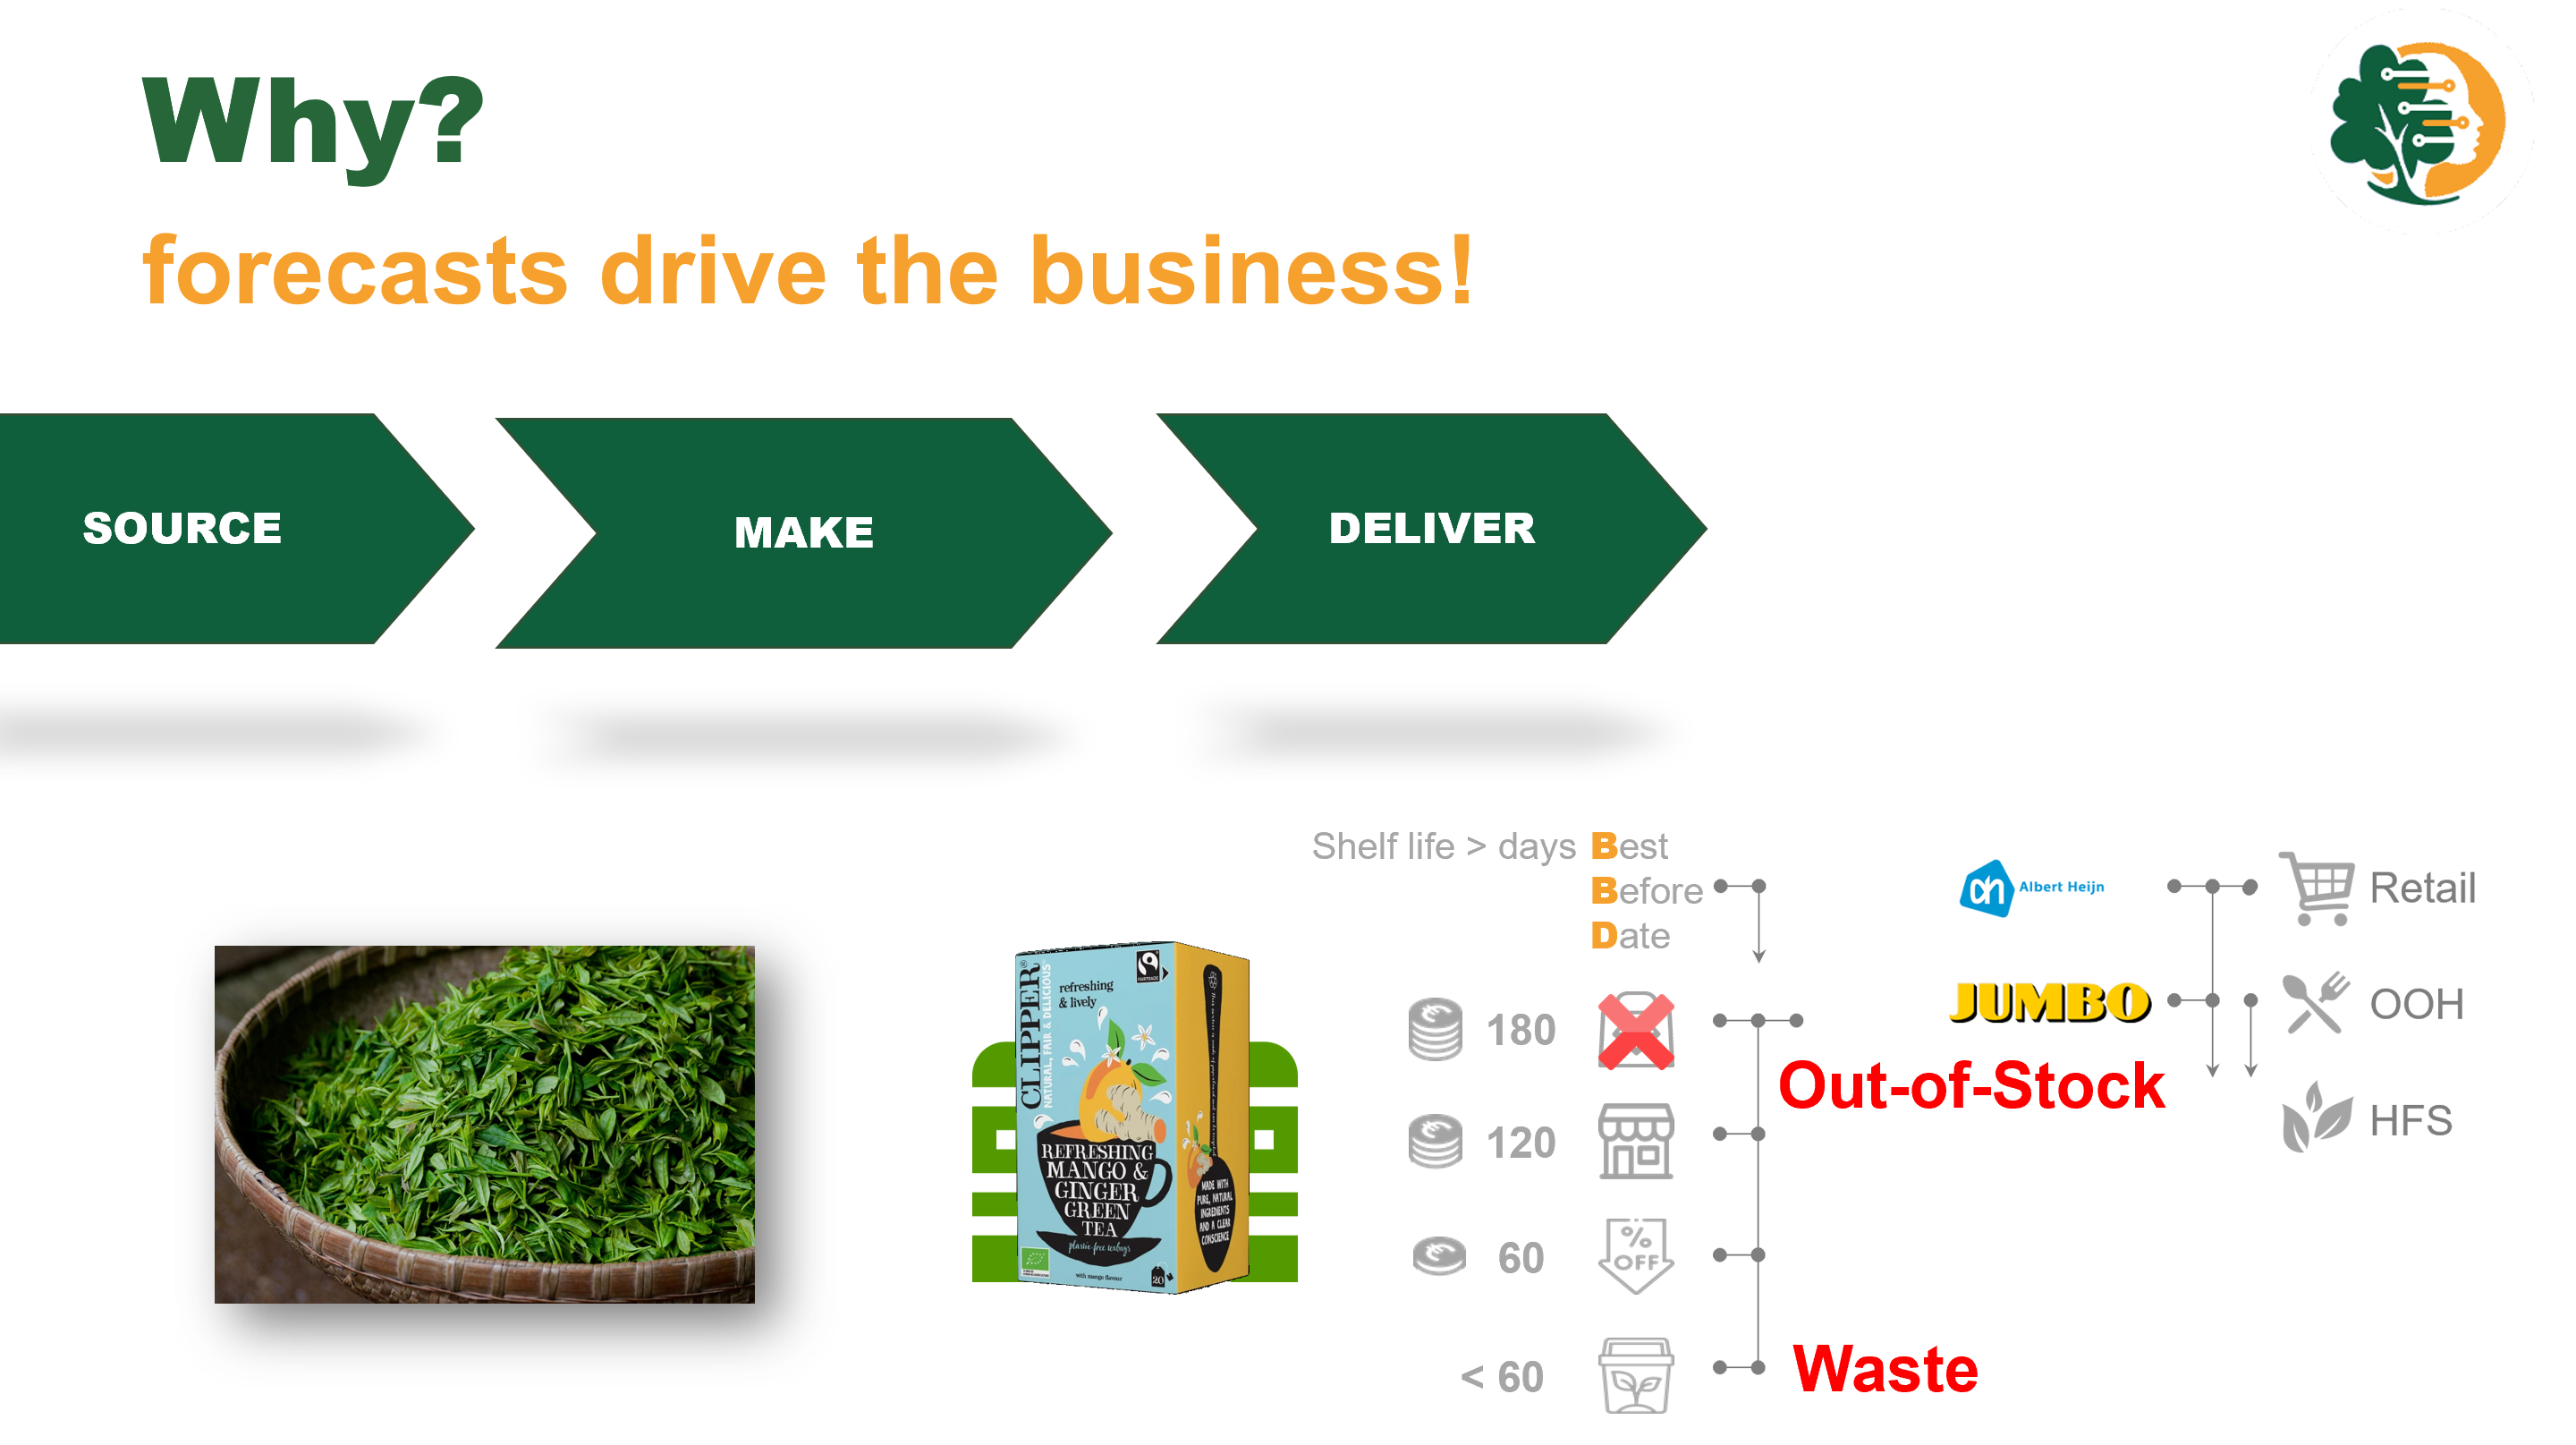
\includegraphics[keepaspectratio]{nb/../images/bu_why.png}}

\end{figure}%

See Figure Figure~\ref{fig-bu-why} for the thumbnail overview.

\chapter{Data Pipelines}\label{data-pipelines}

\chapter{scenario:}\label{scenario}

Dataset Size:

\begin{itemize}
\tightlist
\item
  400 MB in CSV format.
\item
  15 MB in Parquet format.
\end{itemize}

Data Access and Querying:

Happens once when the application starts. Needs to be quick to minimize
user wait time. No data is written to disk during application use; data
is only saved when the application exits. Data Manipulation:

Performed in-memory using R and Python. Requires fast execution.
Consideration:

You like the idea of using Feather for its fast data loading. You're
considering incorporating DuckDB to make the solution more scalable,
despite minimal immediate benefits. Acknowledge that adding DuckDB
introduces additional complexity.

Architecture: Architecture is about the design and setup, provides the
framework and tools. This refers to the high-level structure of your
system. It encompasses the selection of components, technologies,
formats, and how they are organized and interact with each other.
Architecture lays the foundation for your system's capabilities,
scalability, and performance.

Workflow: Workflow is about the execution and processes, defines the
processes and procedures using those tools. This pertains to the
sequence of operations or processes that are carried out using the
architectural components. It describes the specific steps taken to
achieve your objectives, detailing how data and tasks flow through the
system.

\section{Work Flow \& Architecture :}\label{work-flow-architecture}

Need for a a robust, scalable and future-proof architecture with the
flexibility to adapt as the data sets evolves, all while maintaining
excellent performance and usability.

\begin{itemize}
\tightlist
\item
  Need for fast startup and in-memory processing.
\item
  Scalable for future growth
\item
  Minimal in complexity, leveraging familiar tools and lightweight
  components.
\end{itemize}

Vertically Scalable: The architecture leverages your node's 24 GB of
memory effectively, with room for growth by upgrading hardware (e.g.,
adding more RAM or CPU cores).

Low Complexity Overhead:

DuckDB introduces minimal complexity since it integrates seamlessly with
both R and Python. SQL provides a familiar and powerful tool for
managing data subsets, making the workflow easy to maintain. Prepared
for Growth:

The combination of Feather and DuckDB ensures you can handle current and
moderate future data sizes efficiently. For substantial growth, DuckDB
can work with Parquet files or other scalable formats with minimal
changes. Optimized for Performance:

Feather ensures fast data access at startup. DuckDB allows efficient
on-disk querying to reduce memory overhead, ensuring smooth performance
even as datasets grow.

\subsection{}\label{section}

This workflow is ideal when working with datasets that are manageable in
size and can be fully loaded into memory for analysis. Incorporating
DuckDB adds the flexibility of SQL querying, which can be advantageous
for preprocessing data before intensive computations. The use of Feather
format ensures fast data loading, which is important for applications
where user wait time during startup should be minimized.

If your dataset grows or your scalability needs change, you might need
to adjust the workflow accordingly, possibly by switching to Parquet
files and leveraging DuckDB's capabilities to handle larger datasets
more efficiently.

Architecture

Scalability:

\begin{enumerate}
\def\labelenumi{\arabic{enumi}.}
\item
  adjust your SQL queries to limit the data loaded into memory, ensuring
  your application remains performant.
\item
  scale vertically with increased RAM and CPU cores to manage larger
  Feather files and more complex algorithms without architectural
  changes.
\end{enumerate}

Performance:

\begin{itemize}
\tightlist
\item
  Feather enables fast reads for smaller datasets during startup.
\item
  DuckDB efficiently handles larger datasets by querying on disk and
  loading only the necessary data into memory.
\end{itemize}

\subsection{Data Stageing}\label{data-stageing}

\begin{enumerate}
\def\labelenumi{\arabic{enumi}.}
\tightlist
\item
  D00: contains the BW OpenHub Export, CSV - same as AL11
\end{enumerate}

\subsection{Data Ingestion:}\label{data-ingestion}

Occurs once a month, converting CSV to Parquet (or another format).
header is added and stored in D01

\subsection{Data Access and Querying:}\label{data-access-and-querying}

\begin{itemize}
\tightlist
\item
  Data is imported into R data.table objects via DuckDB, which reads the
  stored files.
\item
  Queries are often simple SQL SELECT statements on one table or basic
  INNER JOINs.
\item
  The same SQL queries are used to import data into Python using Polars
  via DuckDB.
\end{itemize}

\subsection{Data Manipulation:}\label{data-manipulation}

\begin{itemize}
\tightlist
\item
  Further data manipulation in R is done using data.table.
\item
  In Python, data manipulation is performed using Polars.
\end{itemize}

\textbf{Evaluation of Your Proposed Workflow}

Given your familiarity with SQL and DuckDB, and your need for
scalability, your proposed workflow is sound and aligns well with your
goals.

\subsection{\texorpdfstring{\textbf{Advantages of Your
Workflow}}{Advantages of Your Workflow}}\label{advantages-of-your-workflow}

\begin{enumerate}
\def\labelenumi{\arabic{enumi}.}
\item
  \textbf{Scalability}

  \begin{itemize}
  \tightlist
  \item
    \textbf{Efficient Data Storage:} Parquet files are columnar,
    compressed, and optimized for performance, which is beneficial for
    large datasets.
  \item
    \textbf{Query Optimization:} DuckDB is designed for efficient
    analytical queries, even on large datasets.
  \end{itemize}
\item
  \textbf{Flexibility}

  \begin{itemize}
  \tightlist
  \item
    \textbf{Language Agnostic:} DuckDB can be used within R and Python,
    allowing seamless transition between languages.
  \item
    \textbf{SQL Familiarity:} Your proficiency in SQL means you can
    leverage DuckDB's SQL interface effectively.
  \end{itemize}
\item
  \textbf{Performance}
\end{enumerate}

\begin{itemize}
\tightlist
\item
  \textbf{Fast Query Execution:} DuckDB is optimized for OLAP workloads
  and can execute complex queries quickly.
\item
  \textbf{Direct Parquet Support:} DuckDB can read Parquet files
  directly without the need to load the entire dataset into memory.
\end{itemize}

\begin{enumerate}
\def\labelenumi{\arabic{enumi}.}
\setcounter{enumi}{3}
\tightlist
\item
  \textbf{Integration with R and Python}
\end{enumerate}

\begin{itemize}
\tightlist
\item
  \textbf{R Data.Tables:} You can fetch query results from DuckDB into R
  data.tables, integrating with your existing R codebase.
\item
  \textbf{Python Polars:} Similarly, you can read data into Polars
  DataFrames in Python, which is efficient for data manipulation.
\end{itemize}

\begin{enumerate}
\def\labelenumi{\arabic{enumi}.}
\setcounter{enumi}{4}
\tightlist
\item
  \textbf{Simplified Data Pipeline}
\end{enumerate}

\begin{itemize}
\tightlist
\item
  \textbf{Unified Data Source:} Using DuckDB on top of Parquet files
  centralizes your data access, simplifying data management.
\end{itemize}

\subsection{\texorpdfstring{\textbf{Potential
Disadvantages}}{Potential Disadvantages}}\label{potential-disadvantages}

\begin{enumerate}
\def\labelenumi{\arabic{enumi}.}
\tightlist
\item
  \textbf{Additional Complexity}
\end{enumerate}

\begin{itemize}
\tightlist
\item
  \textbf{Library Dependencies:} Requires installation and management of
  additional libraries (DuckDB, Parquet support in R and Python).
\item
  \textbf{Learning Curve for Integration:} Even though you're familiar
  with DuckDB, integrating it into R and Python workflows may require
  some setup and testing.
\end{itemize}

\begin{enumerate}
\def\labelenumi{\arabic{enumi}.}
\setcounter{enumi}{1}
\item
  \textbf{Overhead of Data Conversion}

  \begin{itemize}
  \tightlist
  \item
    \textbf{Initial Conversion:} Migrating CSV files to Parquet adds an
    extra step in your data ingestion pipeline.
  \item
    \textbf{Data Updates:} If your CSV data updates frequently, you'll
    need to automate the conversion process.
  \end{itemize}
\item
  \textbf{Resource Usage}
\end{enumerate}

\begin{itemize}
\tightlist
\item
  \textbf{Disk Space:} Maintaining both CSV and Parquet files (if not
  deleting the original CSVs) may consume additional storage.
\end{itemize}

\begin{center}\rule{0.5\linewidth}{0.5pt}\end{center}

\textbf{Recommendations and Best Practices}

Given your requirements and skills, your proposed workflow is suitable
and offers several benefits in terms of scalability and flexibility.
Here are some recommendations to optimize your workflow:

\#\#\# \textbf{1. Automate the CSV to Parquet Conversion}

\begin{itemize}
\item
  \textbf{Use Batch Processing:}
\item
  Create scripts in R or Python to automate the conversion of CSV files
  to Parquet.
\item
  \textbf{Leverage DuckDB for Conversion:}

  \begin{itemize}
  \tightlist
  \item
    DuckDB can read CSV files and write Parquet files, allowing you to
    perform the conversion within DuckDB.
  \end{itemize}
\end{itemize}

\begin{Shaded}
\begin{Highlighting}[]
\KeywordTok{COPY}\NormalTok{ (}\KeywordTok{SELECT} \OperatorTok{*} \KeywordTok{FROM} \StringTok{\textquotesingle{}your\_data.csv\textquotesingle{}}\NormalTok{) }\KeywordTok{TO} \StringTok{\textquotesingle{}your\_data.parquet\textquotesingle{}}\NormalTok{ (FORMAT PARQUET);}
\end{Highlighting}
\end{Shaded}

\subsection{\texorpdfstring{\textbf{2. Optimize DuckDB
Usage}}{2. Optimize DuckDB Usage}}\label{optimize-duckdb-usage}

\begin{itemize}
\item
  \textbf{Indexing and Partitioning:}

  \begin{itemize}
  \tightlist
  \item
    While Parquet files do not support traditional indexing, consider
    partitioning your data to improve query performance.
  \end{itemize}
\item
  \textbf{SQL Query Optimization:}

  \begin{itemize}
  \tightlist
  \item
    Use DuckDB's advanced SQL features to optimize queries (e.g., window
    functions, common table expressions).
  \end{itemize}
\end{itemize}

\subsection{\texorpdfstring{\textbf{3. Efficient Data Retrieval into R
and
Python}}{3. Efficient Data Retrieval into R and Python}}\label{efficient-data-retrieval-into-r-and-python}

\begin{itemize}
\item
  \textbf{In R:}

  \begin{itemize}
  \tightlist
  \item
    Use the \texttt{duckdb} package to execute SQL queries and fetch
    results into data.tables.
  \end{itemize}

\begin{Shaded}
\begin{Highlighting}[]
\FunctionTok{library}\NormalTok{(duckdb)}
\NormalTok{con }\OtherTok{\textless{}{-}} \FunctionTok{dbConnect}\NormalTok{(duckdb}\SpecialCharTok{::}\FunctionTok{duckdb}\NormalTok{())}

\CommentTok{\# Query data}
\NormalTok{result }\OtherTok{\textless{}{-}} \FunctionTok{dbGetQuery}\NormalTok{(con, }\StringTok{"SELECT * FROM \textquotesingle{}your\_data.parquet\textquotesingle{} WHERE conditions"}\NormalTok{)}

\CommentTok{\# Convert to data.table}
\FunctionTok{library}\NormalTok{(data.table)}
\NormalTok{dt\_result }\OtherTok{\textless{}{-}} \FunctionTok{as.data.table}\NormalTok{(result)}
\end{Highlighting}
\end{Shaded}
\item
  \textbf{In Python with Polars:}

  \begin{itemize}
  \tightlist
  \item
    Use DuckDB's Python API or integrate with Polars for efficient data
    handling.
  \end{itemize}
\end{itemize}

\begin{Shaded}
\begin{Highlighting}[]
\ImportTok{import}\NormalTok{ duckdb}
\ImportTok{import}\NormalTok{ polars }\ImportTok{as}\NormalTok{ pl}

\CommentTok{\# Execute query and fetch result as Polars DataFrame}
\NormalTok{df }\OperatorTok{=}\NormalTok{ duckdb.query(}\StringTok{"SELECT * FROM \textquotesingle{}your\_data.parquet\textquotesingle{} WHERE conditions"}\NormalTok{).to\_df()}
\NormalTok{pl\_df }\OperatorTok{=}\NormalTok{ pl.from\_pandas(df)}
\end{Highlighting}
\end{Shaded}

\subsection{\texorpdfstring{\textbf{4. Consider Data Volume and Hardware
Resources}}{4. Consider Data Volume and Hardware Resources}}\label{consider-data-volume-and-hardware-resources}

\begin{itemize}
\item
  \textbf{Memory Management:}

  \begin{itemize}
  \tightlist
  \item
    DuckDB processes data efficiently, but ensure your hardware
    resources are adequate for your data size.
  \end{itemize}
\item
  \textbf{Disk I/O:}

  \begin{itemize}
  \tightlist
  \item
    Using Parquet files reduces disk I/O due to compression, but be
    mindful of the storage subsystem performance.
  \end{itemize}
\end{itemize}

\subsection{\texorpdfstring{\textbf{5. Keep Libraries
Updated}}{5. Keep Libraries Updated}}\label{keep-libraries-updated}

\begin{itemize}
\item
  \textbf{Stay Current:}

  \begin{itemize}
  \tightlist
  \item
    Ensure that you are using the latest versions of DuckDB, R packages,
    and Python libraries to benefit from performance improvements and
    bug fixes.
  \end{itemize}
\end{itemize}

\subsection{\texorpdfstring{\textbf{6. Handle Updates and Data
Versioning}}{6. Handle Updates and Data Versioning}}\label{handle-updates-and-data-versioning}

\begin{itemize}
\item
  \textbf{Incremental Updates:}

  \begin{itemize}
  \tightlist
  \item
    If your data updates incrementally, design your pipeline to handle
    partial updates rather than reprocessing entire datasets.
  \end{itemize}
\item
  \textbf{Data Version Control:}

  \begin{itemize}
  \tightlist
  \item
    Implement versioning for your Parquet files to track changes over
    time.
  \end{itemize}
\end{itemize}

\subsection{\texorpdfstring{\textbf{7. Monitor Performance and
Adjust}}{7. Monitor Performance and Adjust}}\label{monitor-performance-and-adjust}

\begin{itemize}
\item
  \textbf{Benchmarking:}

  \begin{itemize}
  \tightlist
  \item
    Regularly benchmark query performance to identify bottlenecks.
  \end{itemize}
\item
  \textbf{Adjust Strategy:}

  \begin{itemize}
  \tightlist
  \item
    Based on performance metrics, adjust partitioning schemes, query
    strategies, or hardware resources as needed.
  \end{itemize}
\end{itemize}

\begin{center}\rule{0.5\linewidth}{0.5pt}\end{center}

\textbf{Conclusion}

Your proposed workflow of migrating CSV files to Parquet, using DuckDB
for querying, and integrating with R and Python is a robust solution
that addresses your needs for scalability and flexibility. Given your
familiarity with SQL and DuckDB, and the fact that you possess the
necessary skills to manage the additional complexity, this approach is
well-suited to your situation.

\textbf{Benefits of Your Workflow:}

\begin{itemize}
\item
  \textbf{Scalable Data Processing:}
\item
  Efficient handling of large datasets through Parquet and DuckDB.
\item
  \textbf{Flexibility Across Languages:}

  \begin{itemize}
  \tightlist
  \item
    Seamless data access in both R and Python without data format
    conversion issues.
  \end{itemize}
\item
  \textbf{Performance Optimization:}

  \begin{itemize}
  \tightlist
  \item
    Faster query execution and data retrieval due to optimized storage
    and processing.
  \end{itemize}
\end{itemize}

\textbf{Key Actions Moving Forward:}

\begin{enumerate}
\def\labelenumi{\arabic{enumi}.}
\tightlist
\item
  \textbf{Set Up Automated Data Pipelines:}
\end{enumerate}

\begin{itemize}
\tightlist
\item
  Automate the conversion from CSV to Parquet to ensure consistency and
  save time.
\end{itemize}

\begin{enumerate}
\def\labelenumi{\arabic{enumi}.}
\setcounter{enumi}{1}
\tightlist
\item
  \textbf{Optimize Queries:}
\end{enumerate}

\begin{itemize}
\tightlist
\item
  Utilize DuckDB's full SQL capabilities to write efficient queries for
  your analysis.
\end{itemize}

\begin{enumerate}
\def\labelenumi{\arabic{enumi}.}
\setcounter{enumi}{2}
\item
  \textbf{Integrate Smoothly with R and Python:}

  \begin{itemize}
  \tightlist
  \item
    Establish standard functions or scripts in both environments to
    interact with DuckDB, minimizing repetitive code.
  \end{itemize}
\item
  \textbf{Monitor and Iterate:}

  \begin{itemize}
  \tightlist
  \item
    Keep an eye on performance metrics and be ready to adjust your
    approach as your dataset grows or changes.
  \end{itemize}
\end{enumerate}

\begin{center}\rule{0.5\linewidth}{0.5pt}\end{center}

\textbf{Additional Considerations}

\begin{itemize}
\item
  \textbf{Community and Support:}

  \begin{itemize}
  \tightlist
  \item
    DuckDB is actively developed, and there is a growing community.
    Utilize resources like documentation and forums when needed.
  \end{itemize}
\item
  \textbf{Testing and Validation:}

  \begin{itemize}
  \tightlist
  \item
    As with any data pipeline, thoroughly test each component to ensure
    data integrity and correctness.
  \end{itemize}
\item
  \textbf{Security and Access Control:}

  \begin{itemize}
  \tightlist
  \item
    If working in a multi-user environment, consider how data access and
    permissions are managed.
  \end{itemize}
\end{itemize}

\begin{center}\rule{0.5\linewidth}{0.5pt}\end{center}

\textbf{Final Thoughts}

Your willingness to embrace additional complexity due to your skill set
positions you well to benefit from this workflow. By combining the
strengths of Parquet's efficient data storage and DuckDB's powerful
query engine, you can achieve a scalable and flexible data analysis
environment.

Should you need further assistance or have more questions as you
implement this workflow, feel free to reach out. I'm here to help ensure
your data processing is as efficient and effective as possible.

\chapter{Data Stageing}\label{data-stageing-1}

data lake design pattern: Bronze-Silver-Gold structure data according to
its level of processing and readiness for use.

Bronze Layer (Raw Data): Contains raw data as it was ingested from the
source systems. This data is typically in its original format and
unprocessed.

Silver Layer (Cleaned and Conformed Data): Contains data that has been
cleansed, filtered, and possibly enriched. This data is ready for
further processing or analysis but is not yet aggregated or modeled.

Gold Layer (Curated Data): Contains data that has been transformed into
business-level aggregates, models, or reports. This is the data used by
analysts, data scientists, or applications for decision-making.

\chapter{Modelling}\label{modelling}

Modelling subtitle

\hfill\break

\begin{figure}

\caption{\label{fig-bu-why}Why forecasting?\\
The forecast drives the business!}

\pandocbounded{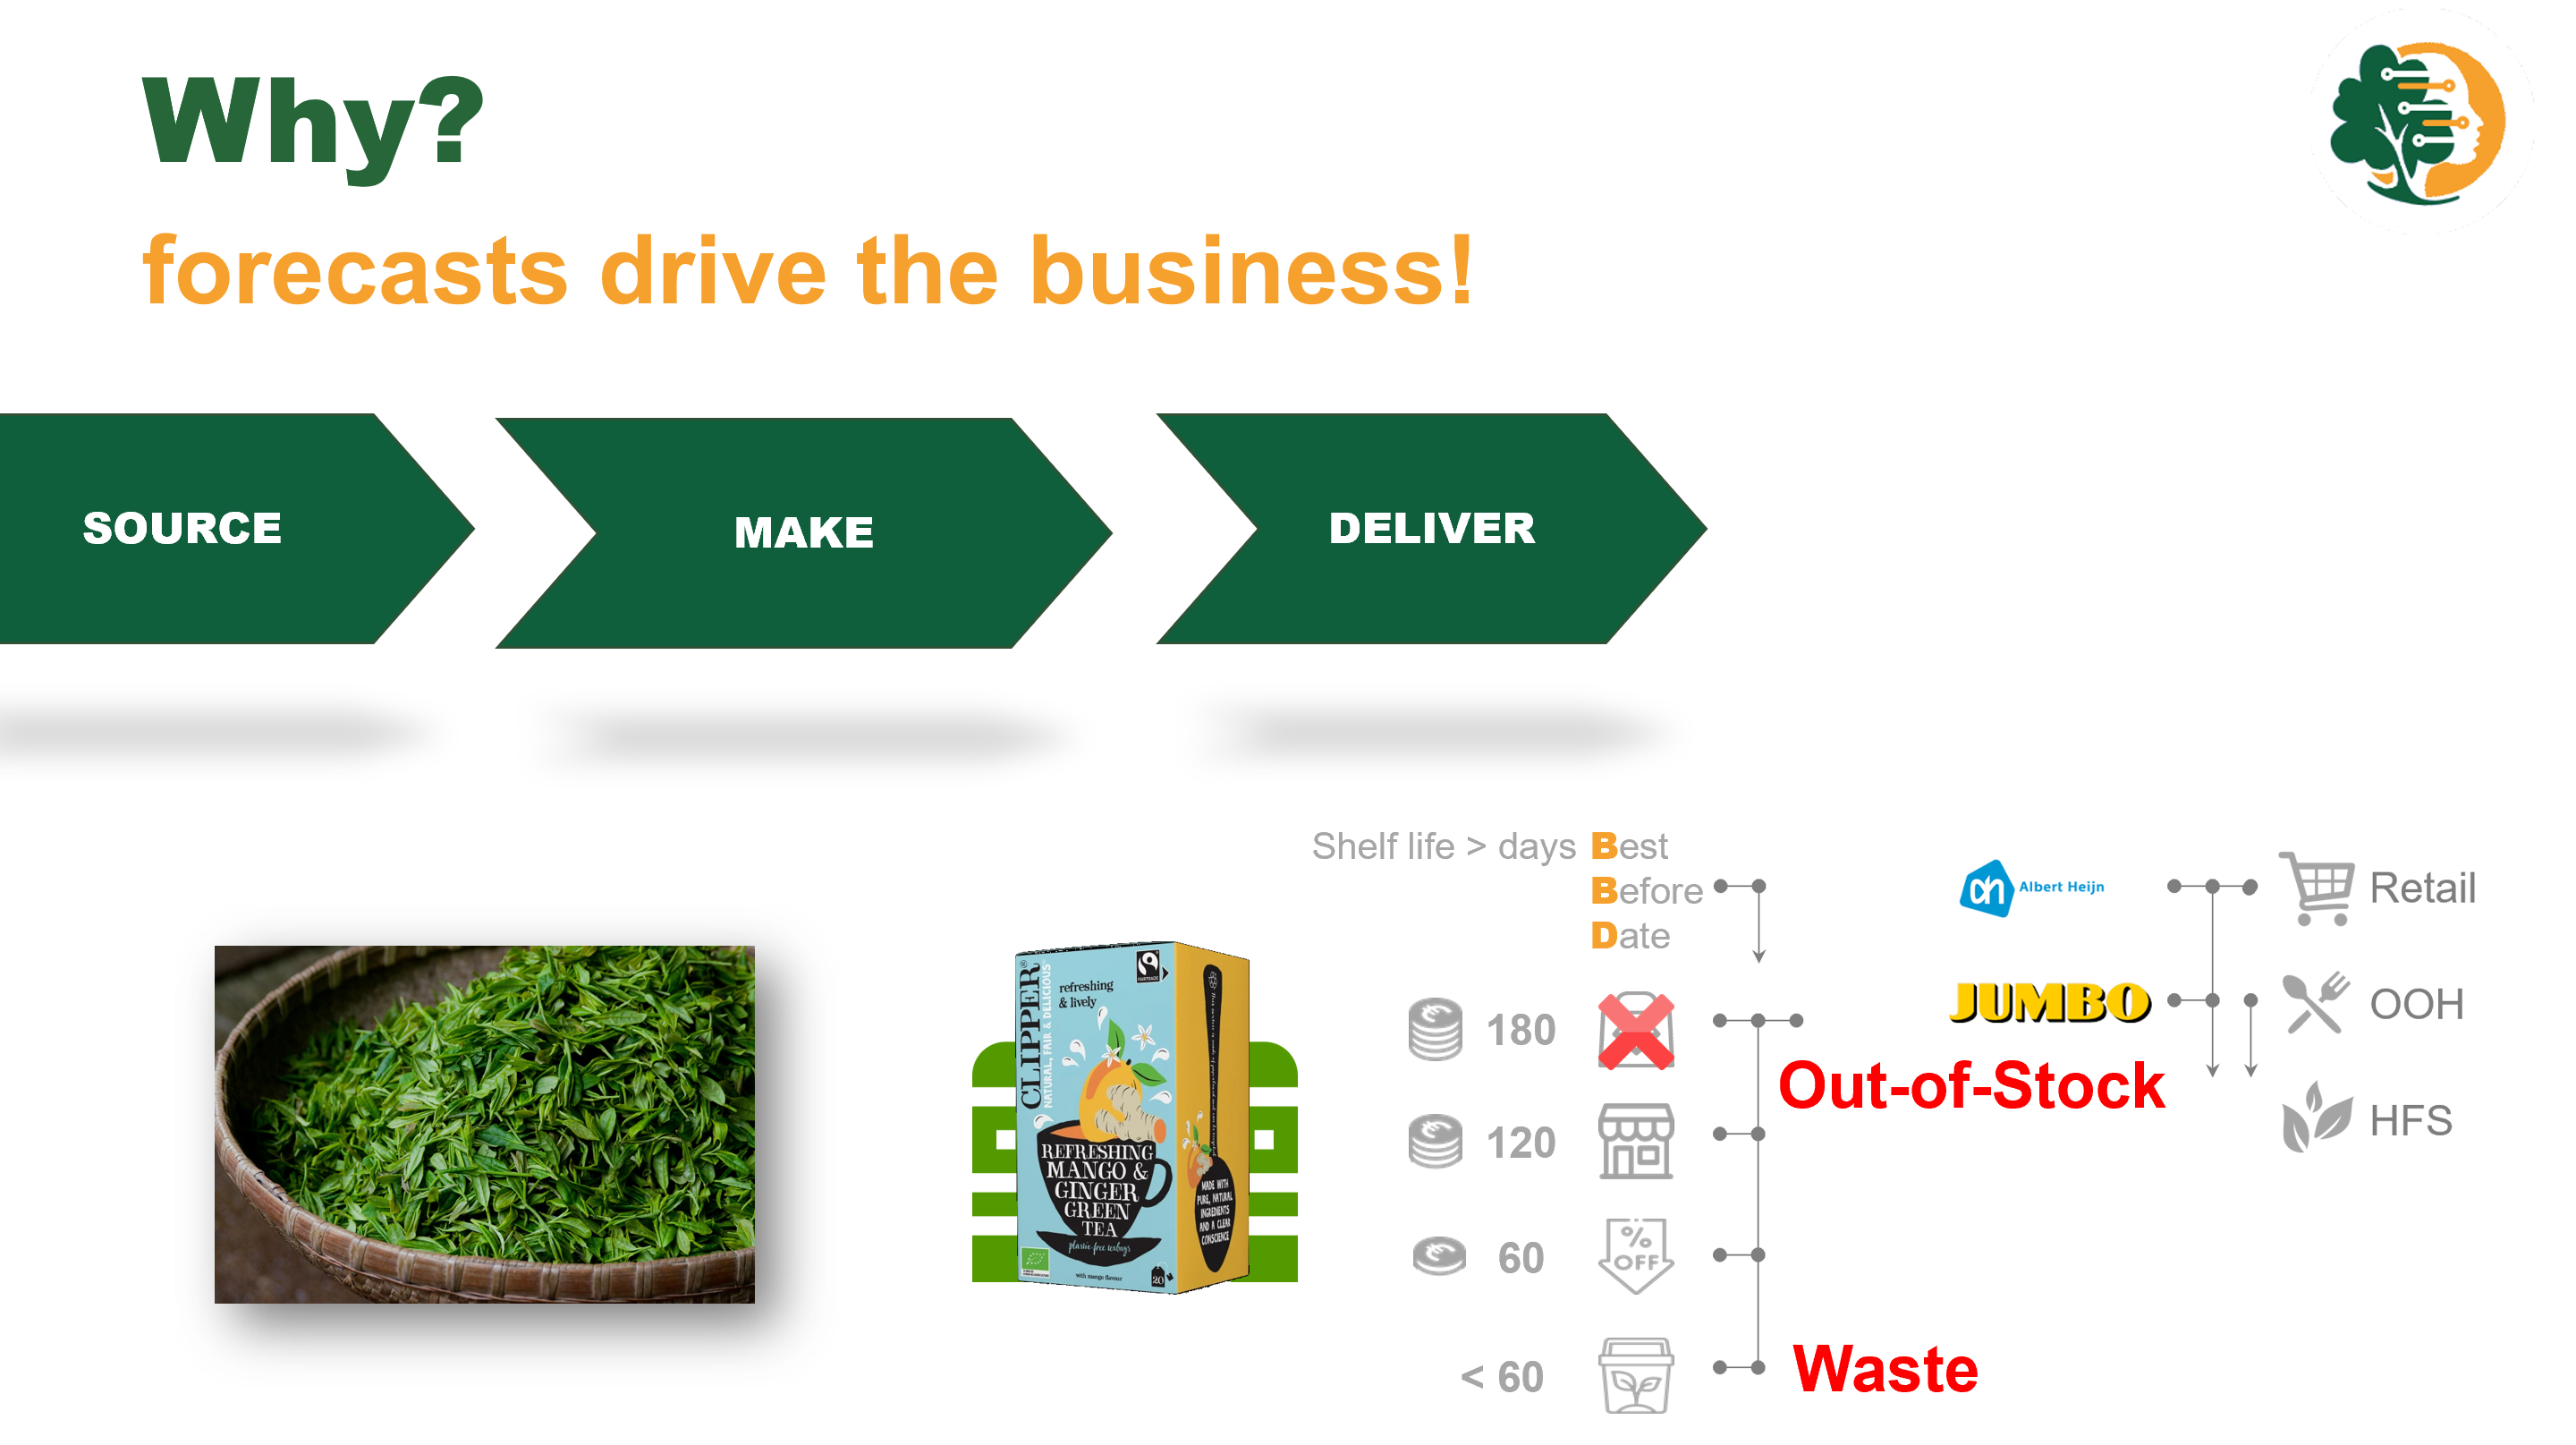
\includegraphics[keepaspectratio]{nb/../images/bu_why.png}}

\end{figure}%

See Figure Figure~\ref{fig-bu-why} for the thumbnail overview.

\section{blackbox models}\label{blackbox-models}

\section{whitebox models}\label{whitebox-models}

6.1. Literature Review / Similar Models - comprehensive overview of the
state of the art in machine learning, including the latest algorithms, -
insight into the performance of different algorithms and techniques on
similar types of data. (avoid wasting time on models that are unlikely
to perform well.)

\subsection{Model Selection}\label{model-selection}

different models have different strengths and weaknesses and are
suitable for different types of data and problems. achieve the best
possible performance and maximize the impact

avoid overfitting a trade-off between the simplicity and flexibility
(robustness)

model performance - only article hierarchy - article and customer
hierarchy

Cross-validation is a method for evaluating the performance of a model
on a validation dataset. This involves dividing the data into k folds,
training the model on k-1 folds, and evaluating the performance on the
remaining fold. This process is repeated k times, with each fold serving
as the validation set once, and the results are averaged to obtain a
final performance score. This method provides a more reliable estimate
of the model's performance, as it uses all of the data for training and
evaluation.

algorithm - handle teh specific characteristics of teh data - balance
performance and interpretability - memory and processing power

\begin{itemize}
\tightlist
\item
  validity -\textgreater{} fa \& prediction intervals
\item
  robustness -\textgreater{}
\item
  transparency -\textgreater{}
\end{itemize}

\chapter*{Appendix}\label{appendix-1}
\addcontentsline{toc}{chapter}{Appendix}

\markboth{Appendix}{Appendix}

\chapter{Evaluation}\label{evaluation-1}

Evaluation subtitle

\hfill\break

\section{Evaluate Results}\label{evaluate-results}

\begin{itemize}
\tightlist
\item
  explainability
\end{itemize}

\subsection{Assessment of Data Mining Results w.r.t. Business Success
Criteria}\label{assessment-of-data-mining-results-w.r.t.-business-success-criteria}

\begin{itemize}
\item
  how well does the model work on new data?
\item
  For whom does the model not work well?
\end{itemize}

\subsection{Approved Models}\label{approved-models}

\subsection{Review Process}\label{review-process}

\subsection{Review of Process}\label{review-of-process}

\subsection{Determine Next Steps}\label{determine-next-steps}

\subsection{List of Possible Actions}\label{list-of-possible-actions}

\subsection{Decision}\label{decision}

\chapter*{Appendix}\label{appendix-2}
\addcontentsline{toc}{chapter}{Appendix}

\markboth{Appendix}{Appendix}

\chapter{Deployment}\label{deployment-1}

Deployment subtitle

\hfill\break

scalability - distributed techniques - maintenance \& updating the model
- monitoring the model - debugging the model

\chapter{model management}\label{model-management}

\begin{itemize}
\tightlist
\item
  model versioning GIT
\item
  continuous integration/continuous deployment (CI/CD) pipelines.
\end{itemize}

\chapter*{Appendix}\label{appendix-3}
\addcontentsline{toc}{chapter}{Appendix}

\markboth{Appendix}{Appendix}

\chapter{Other}\label{other}

Other sub

\hfill\break

\chapter*{other}\label{other-1}
\addcontentsline{toc}{chapter}{other}

\markboth{other}{other}

\section{Literature}\label{sec-literature_review}

The literature review focuses on the intersection of three fields,
according to the now-ubiquitous Data Science Venn Diagram of
\href{http://drewconway.com/zia/2013/3/26/the-data-science-venn-diagram}{Drew
Conway}.

\section{Business Process}\label{business-process}

\begin{itemize}
\tightlist
\item
  SCOR MODEL A COMPLETE GUIDE - 2020 EDITION, (BLOKDYK, 2019)
\item
  Inventory and production management in supply chains, (Silver et al.,
  2021)
\end{itemize}

\section{Math \& Statistics}\label{math-statistics}

\begin{itemize}
\tightlist
\item
  Forecasting: Principles and Practice (3rd ed), (Hyndman \&
  Athanasopoulos, 2021)
\item
  Demand forecasting best practices, (Vandeput, 2023)
\item
  Data science for supply chain forecasting, (Vandeput, 2021)
\item
  Inventory optimization: models and simulations, (Vandeput, 2020)
\item
  Machine Learning With Boosting: A Beginner's Guide, (Hartshorn, 2017)
\item
  Introduction to conformal prediction with Python, (Molnar, 2023)
\item
  Practical guide to applied conformal prediction in Python, (Manokhin,
  2023)
\item
  SHAP with Python, (O'Sullivan, 2024)
\item
  Introduction to SHAP with Python, (O'Sullivan, 2023)
\item
  Ensemble methods for machine learning, (Kunapuli, 2023)
\end{itemize}

\section{Programming}\label{programming}

\subsection{Python}\label{python}

\begin{itemize}
\tightlist
\item
  Python Crash Course, (Matthes, 2019a)
\item
  Lightning fast forecasting with statistical and econometric models,
  (\emph{Nixtla/statsforecast}, 2024)
\item
  Scalable Machine Learning for Time Series Forecasting,
  (\emph{Nixtla/mlforecast}, 2024)
\item
  Probabilistic hierarchical forecasting with statistical and
  econometric methods, (\emph{Nixtla/hierarchicalforecast}, n.d.)
\item
  TS Features, calculates various features from time series data,
  (\emph{Nixtla/tsfeatures}, 2024)
\end{itemize}

\subsection{R}\label{r}

\begin{itemize}
\tightlist
\item
  R for Data Science, (Wickham, n.d.)
\item
  R forecasting package, (Hyndman {[}aut, cre, cph, Athanasopoulos,
  Bergmeir, et al., 2024)
\item
  R feasts package, (O'Hara-Wild, Hyndman, Wang, Cook, et al., 2024)
\item
  R fable package, (O'Hara-Wild, Hyndman, Wang, implementation), et al.,
  2024)
\end{itemize}

\begin{landscape}

\section{Forecast Use Cases}\label{sec-forecast-use-cases}

\begin{figure}[H]

\caption{Forecast Use Cases}

{\centering 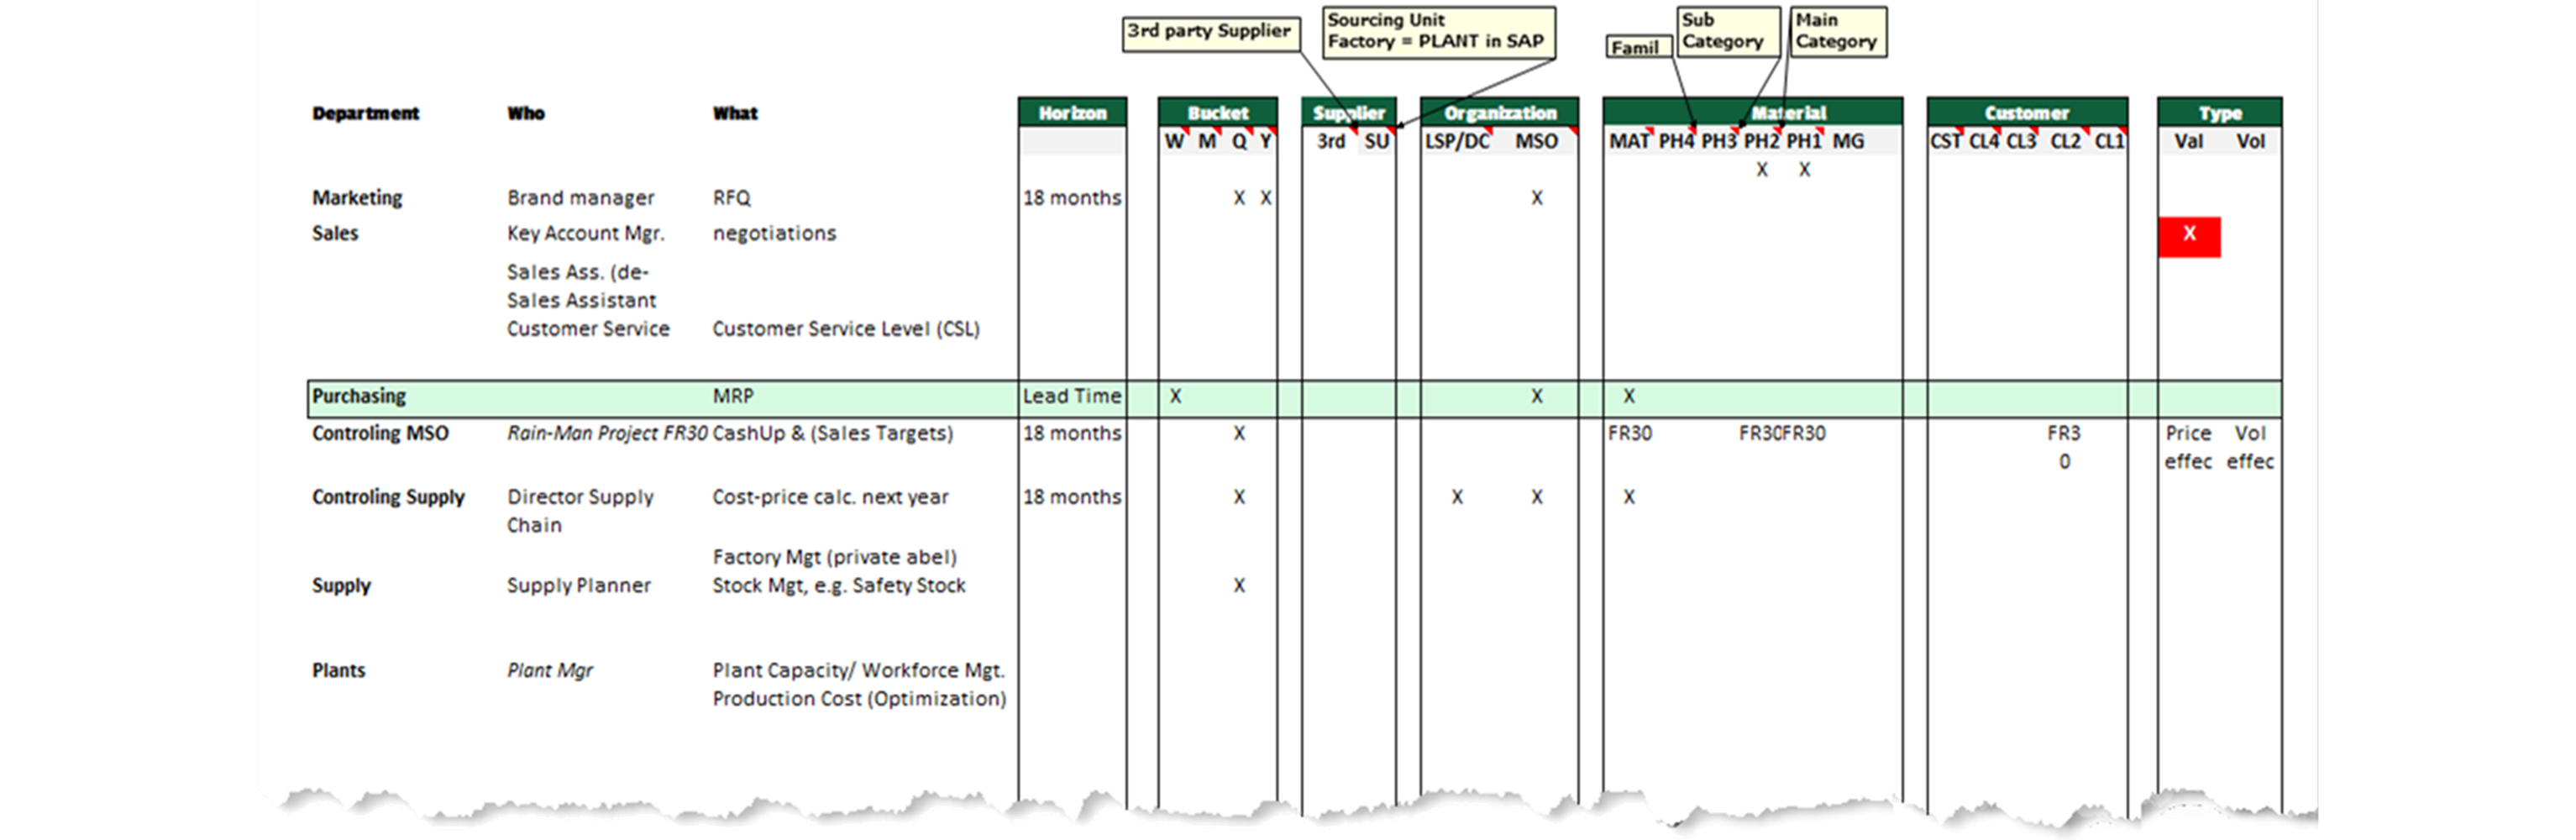
\includegraphics[width=1\linewidth,height=\textheight,keepaspectratio]{nb/../images/forecast_use_cases.png}

}

\end{figure}%

\section{Project Charter}\label{sec-project-charter}

\begin{figure}[H]

\caption{Project Charter}

{\centering 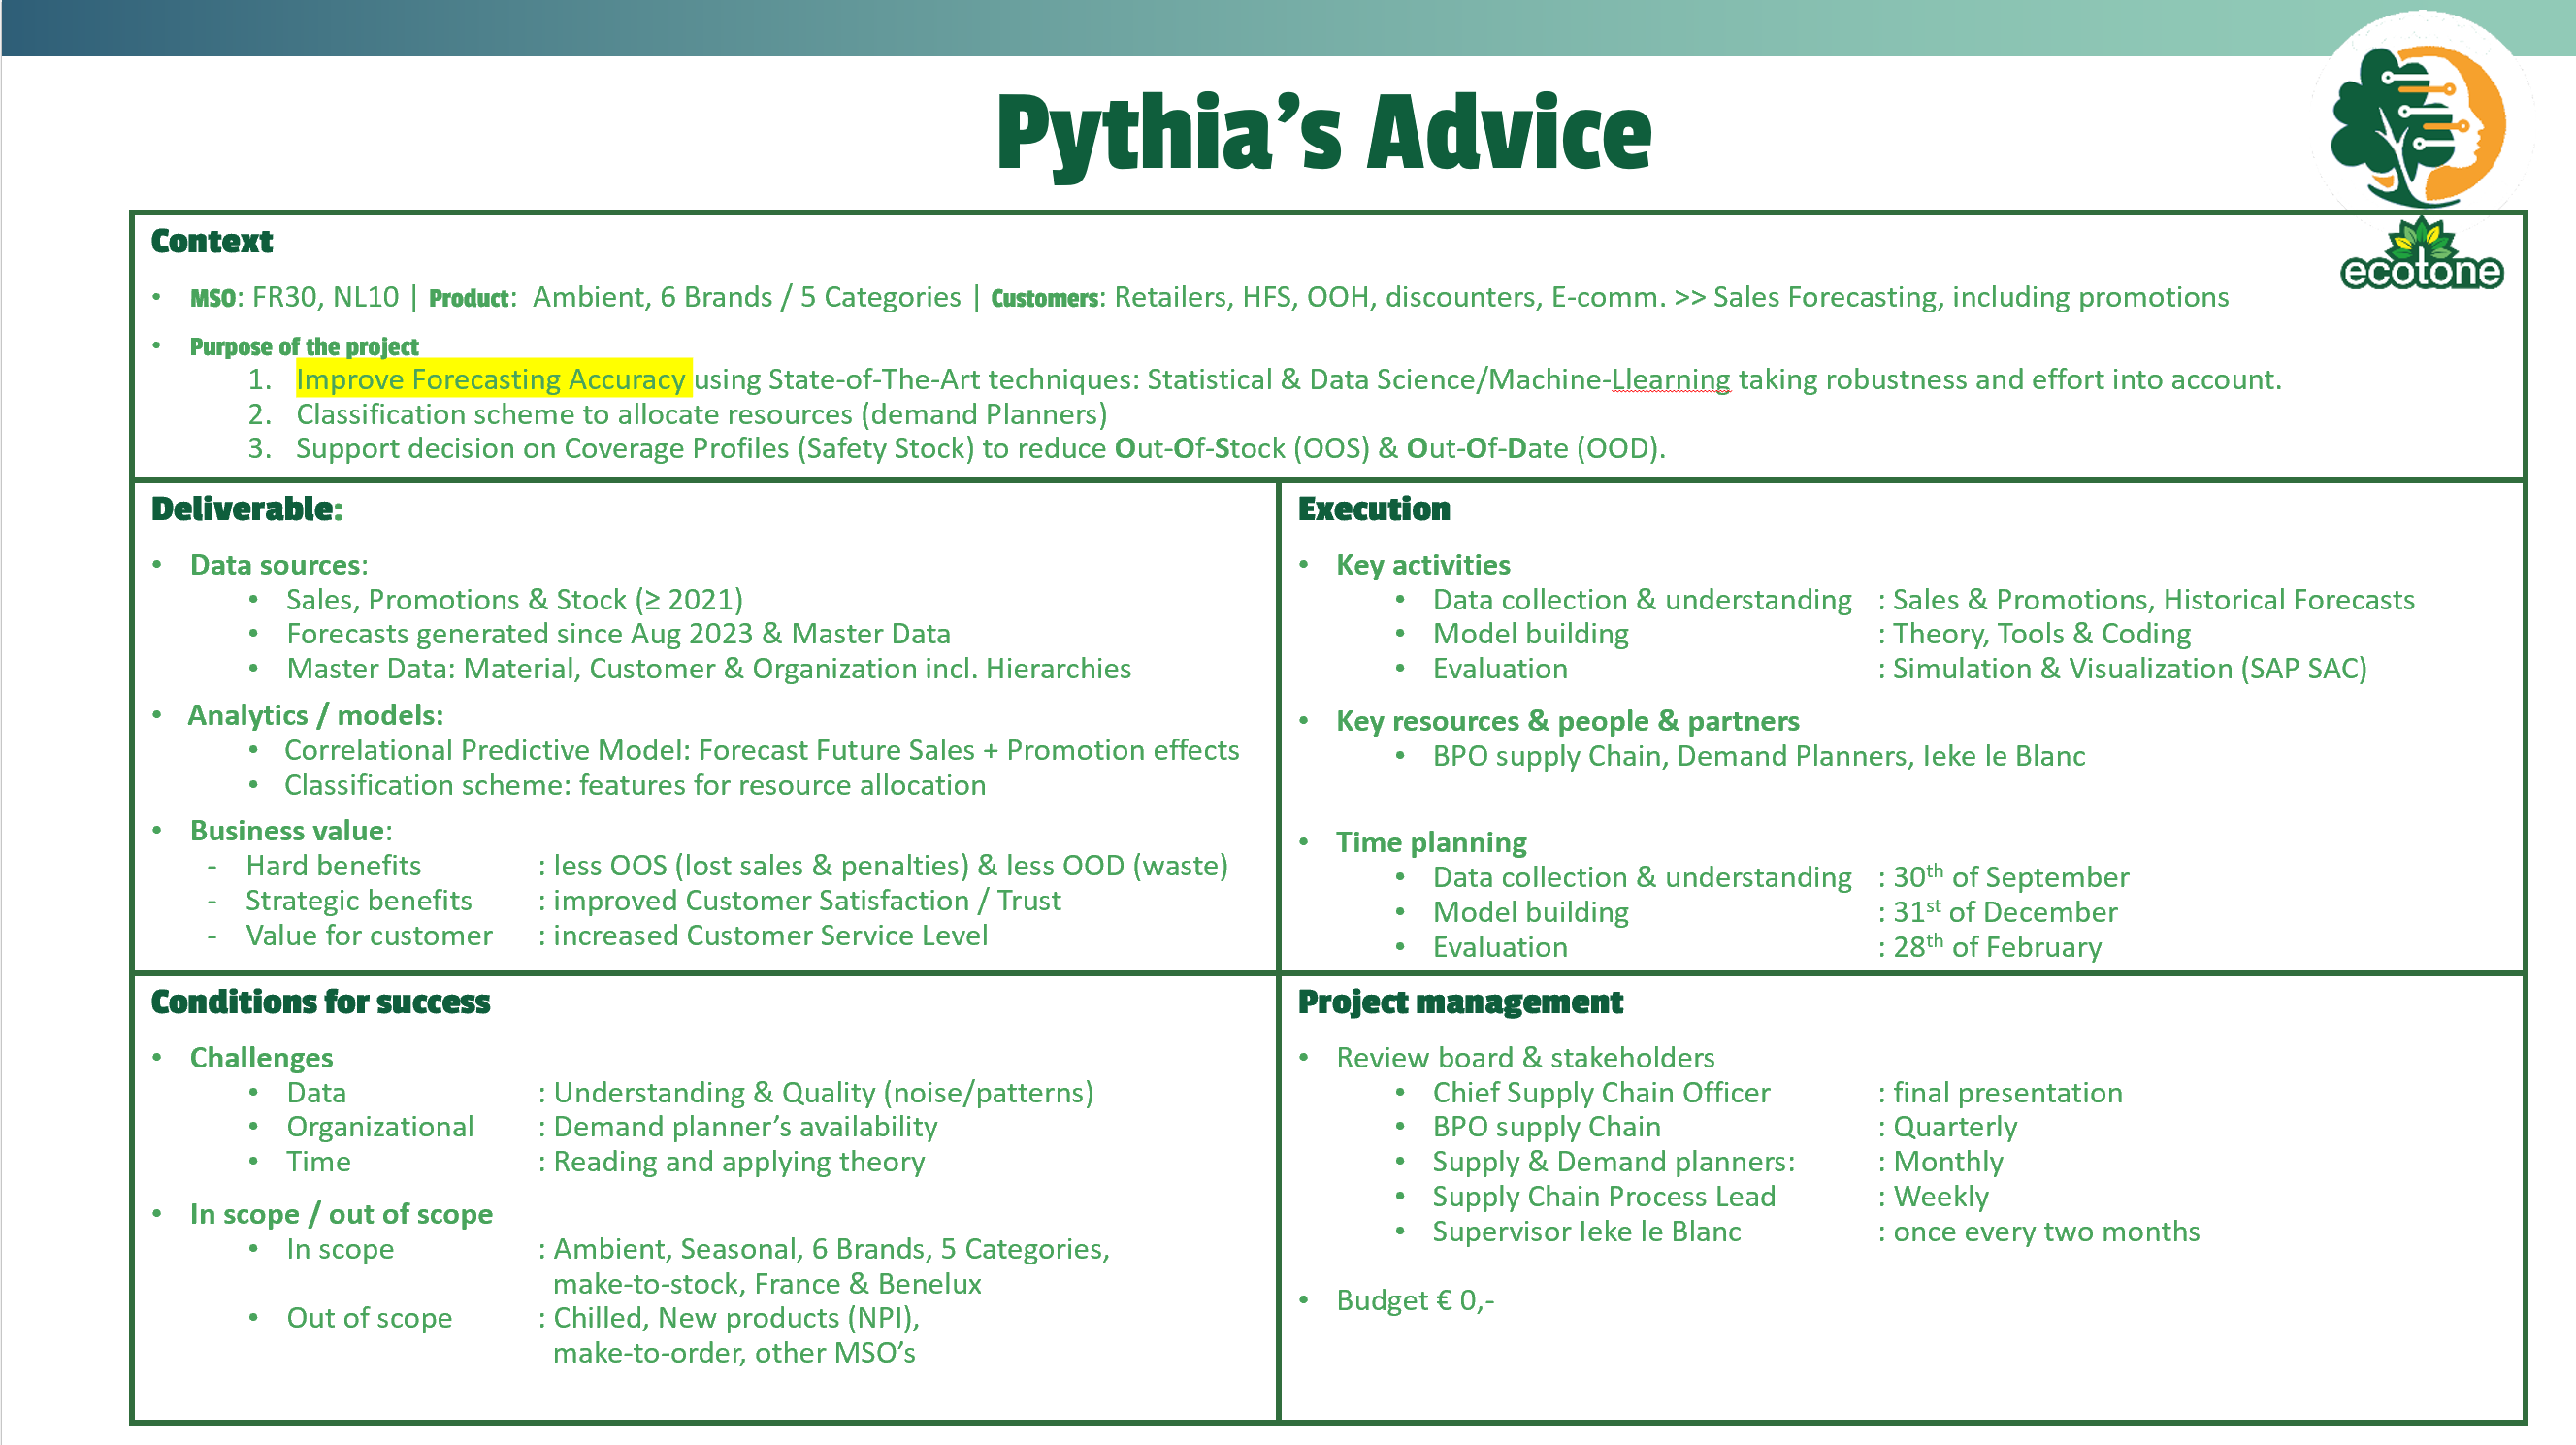
\includegraphics[width=1\linewidth,height=\textheight,keepaspectratio]{nb/../images/project_charter.png}

}

\end{figure}%

\section{Project Plan}\label{sec-project-plan}

\begin{figure}[H]

\caption{Project Plan}

{\centering 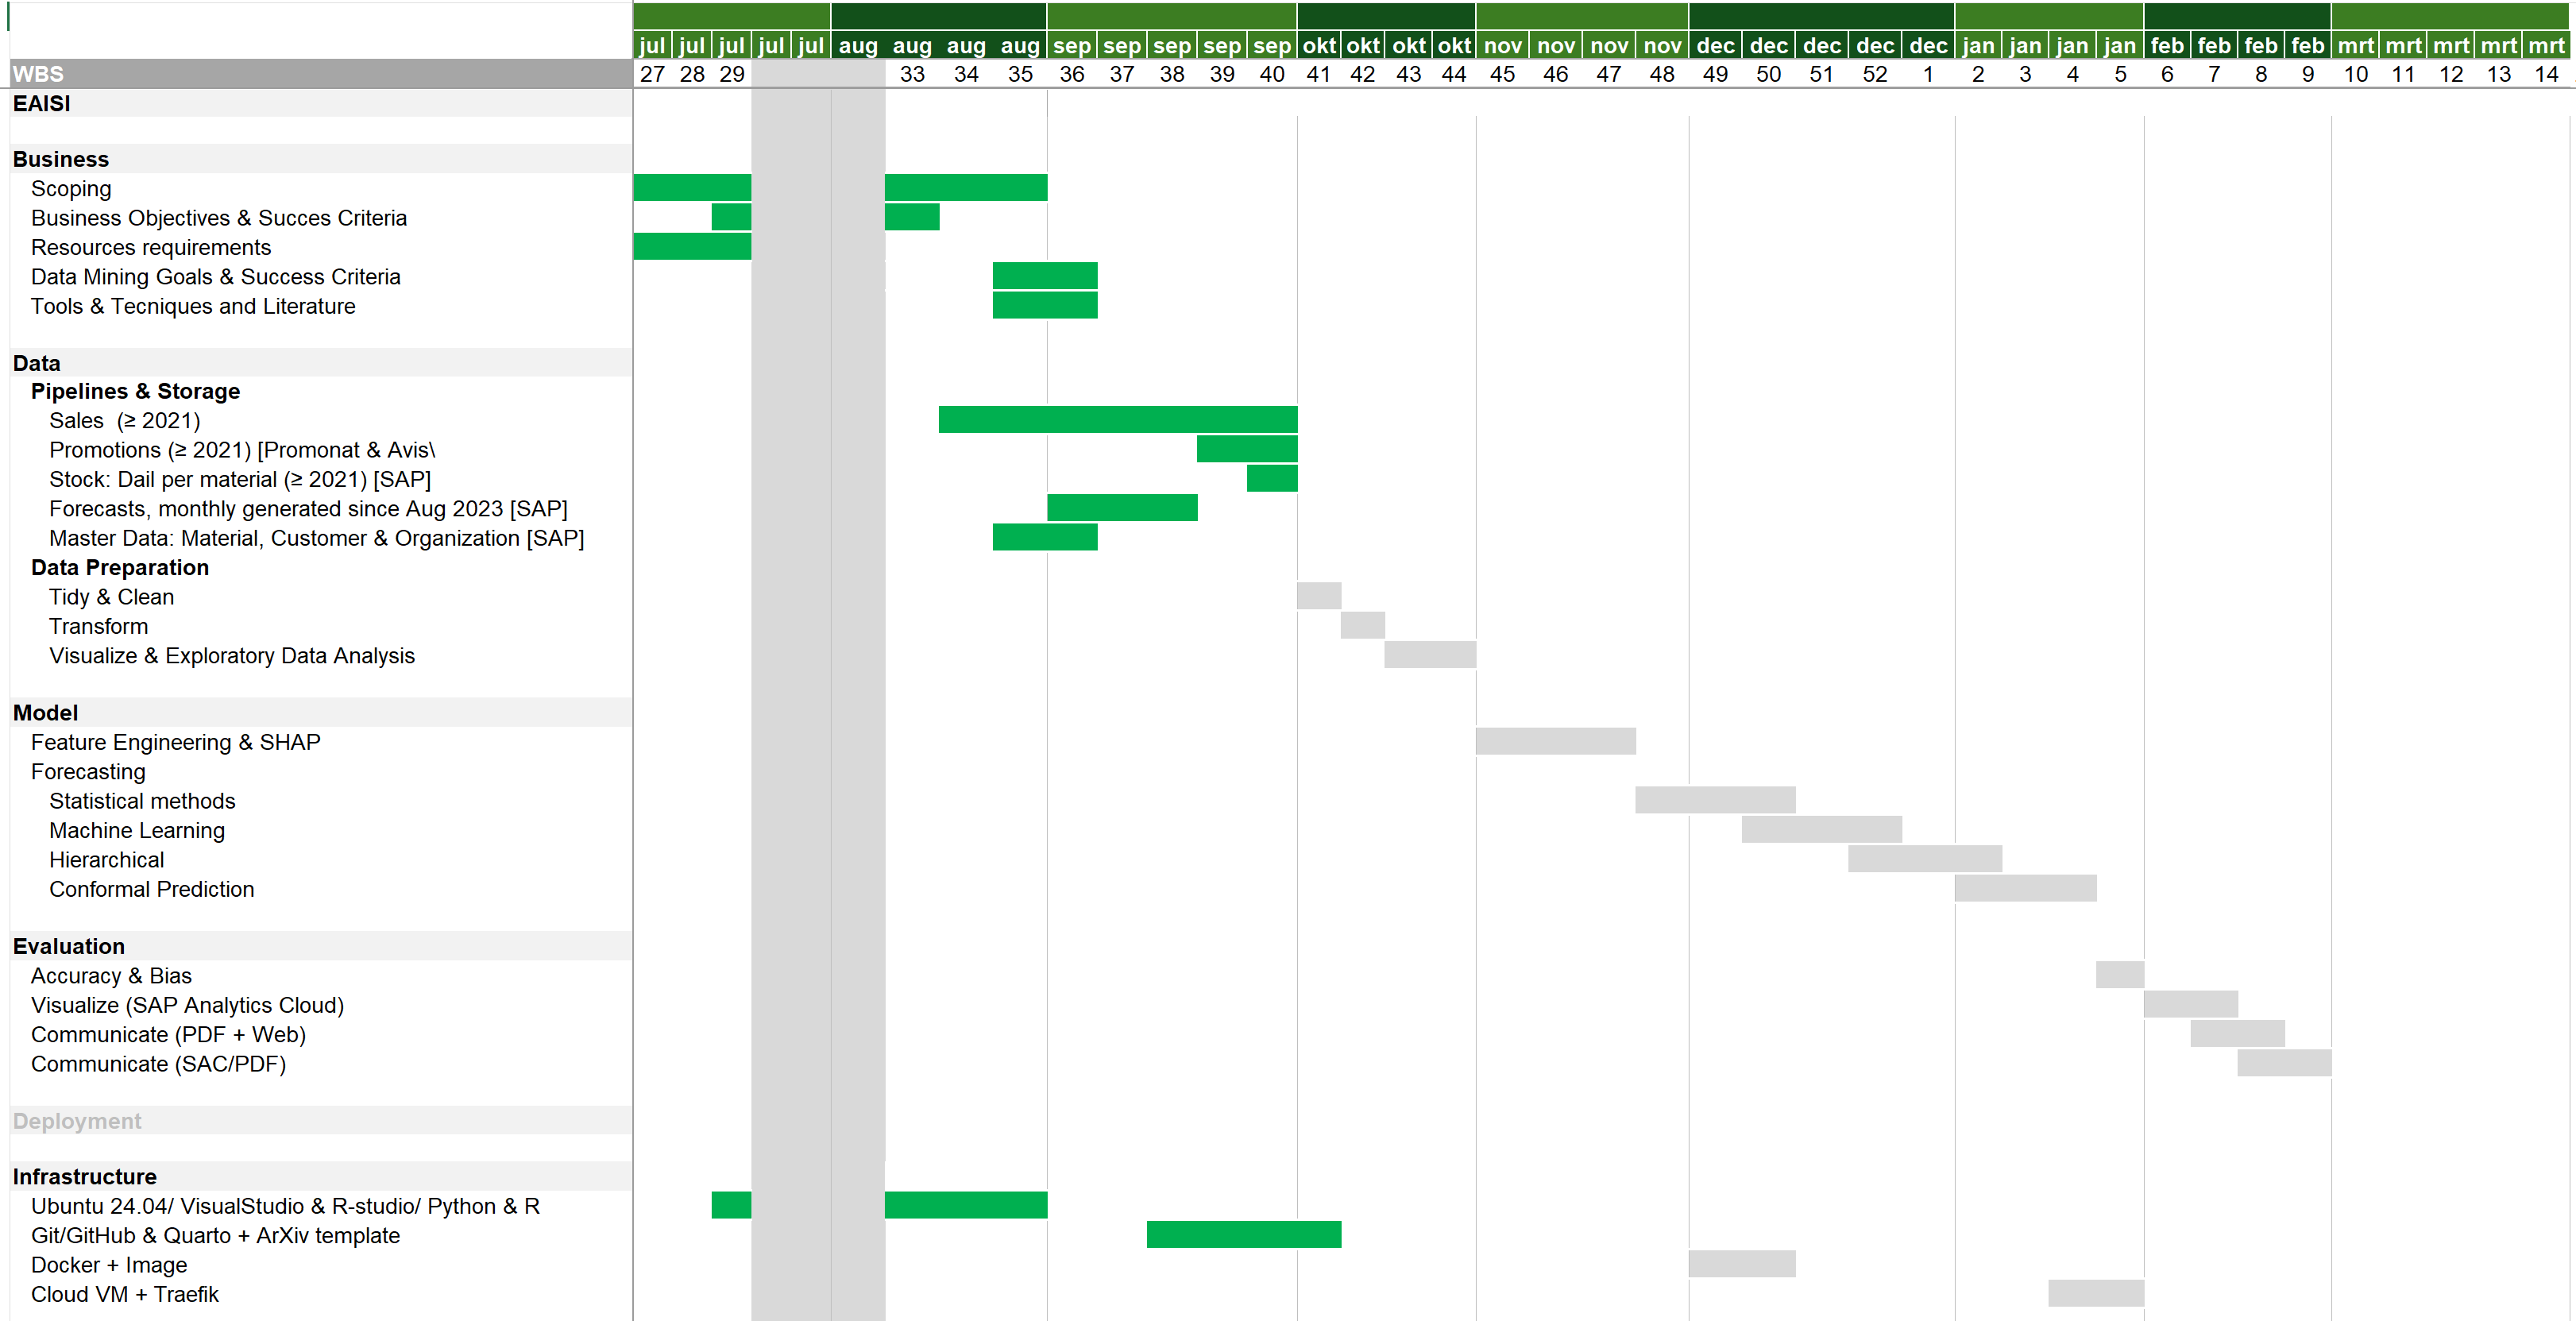
\includegraphics[width=1\linewidth,height=\textheight,keepaspectratio]{nb/../images/project_plan.png}

}

\end{figure}%

\newpage{}

\begin{figure}[H]

\caption{Project Plan}

{\centering 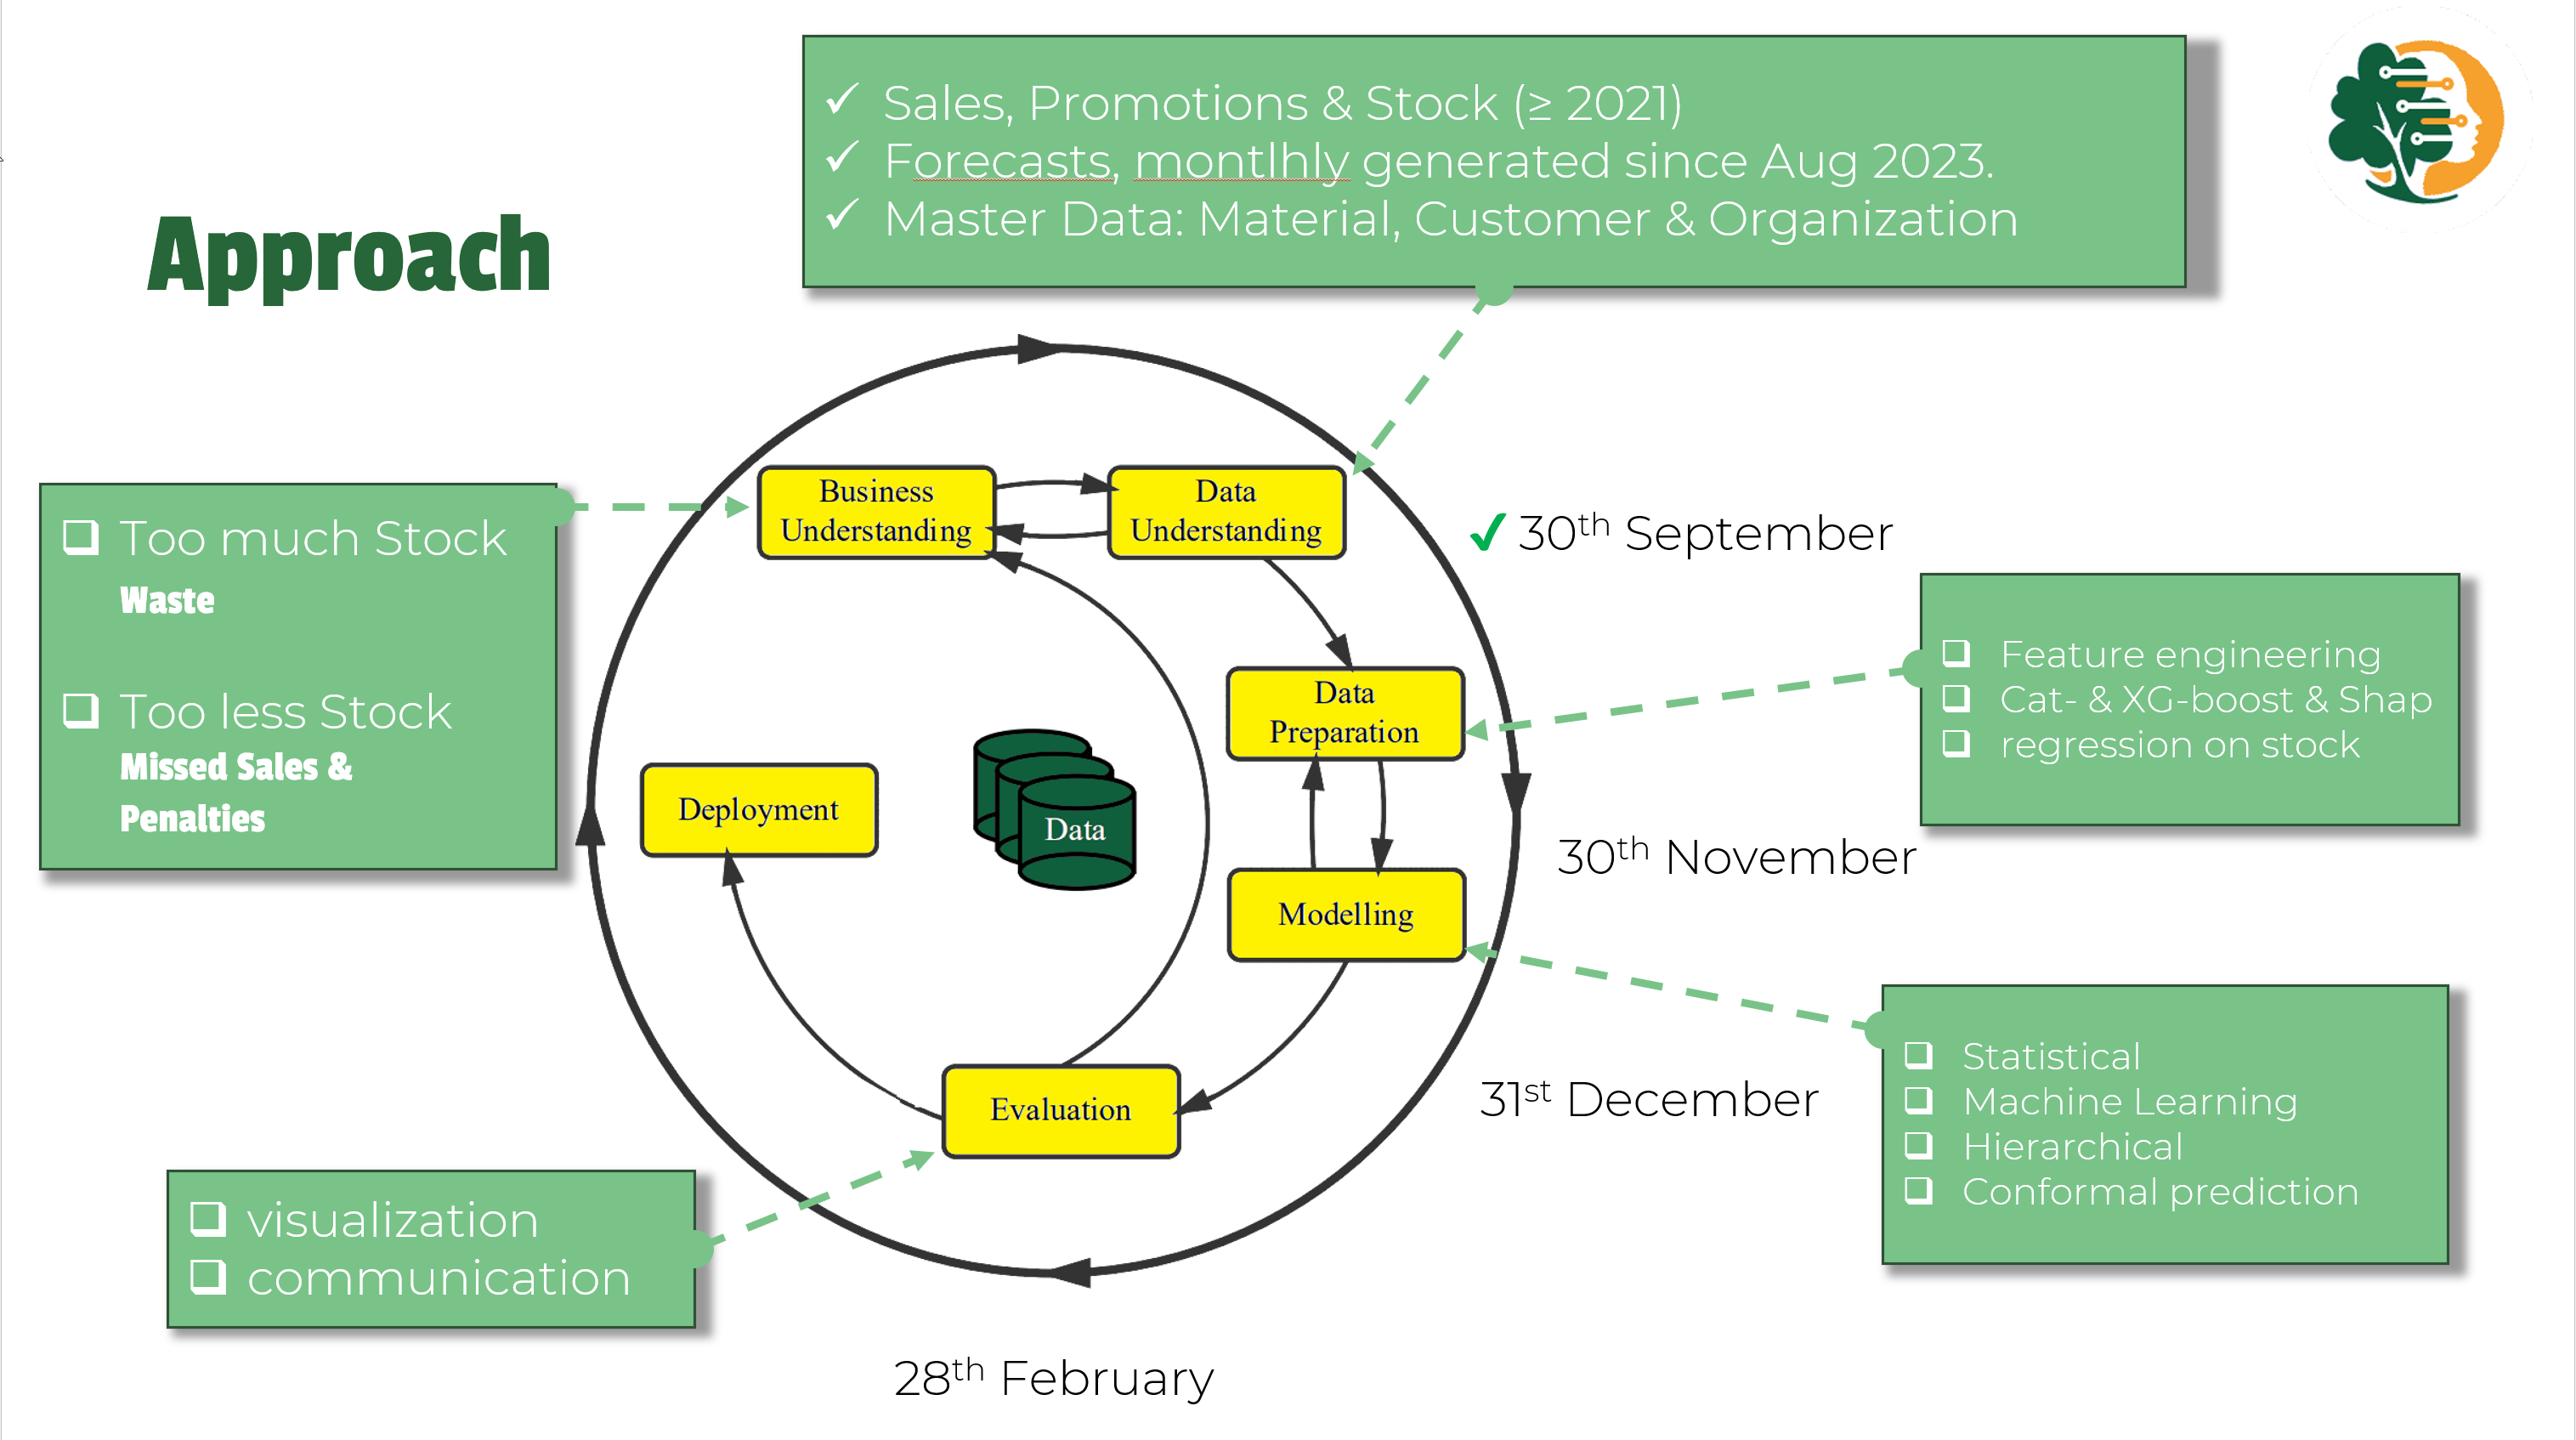
\includegraphics[width=0.8\linewidth,height=\textheight,keepaspectratio]{nb/../images/approach.png}

}

\end{figure}%

\newpage{}

\end{landscape}

\section{EAISI}\label{sec-eaisi}

\subsection{\texorpdfstring{\href{https://academy.eaisi.nl/l/41851394}{Deliverables
\&
requirements}}{Deliverables \& requirements}}\label{deliverables-requirements}

\begin{itemize}
\tightlist
\item
  Clear description of the need / problem / opportunity
\item
  Clear description of the long-term ambition
\item
  Clear focus on what part of this long-term ambition will be taken on
  in the project
\item
  Description of the data science project with the help of a flowdown
  chart and project charter
\item
  Clear description of how the model outcome / analysis results will be
  used (e.g.~who, at what time, in which process, in what way, will use
  the model outcome / analysis results to make a better decision about
  what?) and how this translates into improved KPIs as outlined in the
  flowdown chart
\item
  Substantiated choice for a `performance metric' (i.e.~what should the
  model be good at)
\item
  Clear description of a business case / cost-benefit (no cost!!)
  analysis
\item
  Realistic plan / timeline for how to execute the consecutive CRISP-DM
  phases
\end{itemize}

\chapter{Flow Down}\label{flow-down}

\section{Flow-down}\label{sec-flowdown}

\begin{figure}[H]

\caption{Flowdown Graph}

{\centering 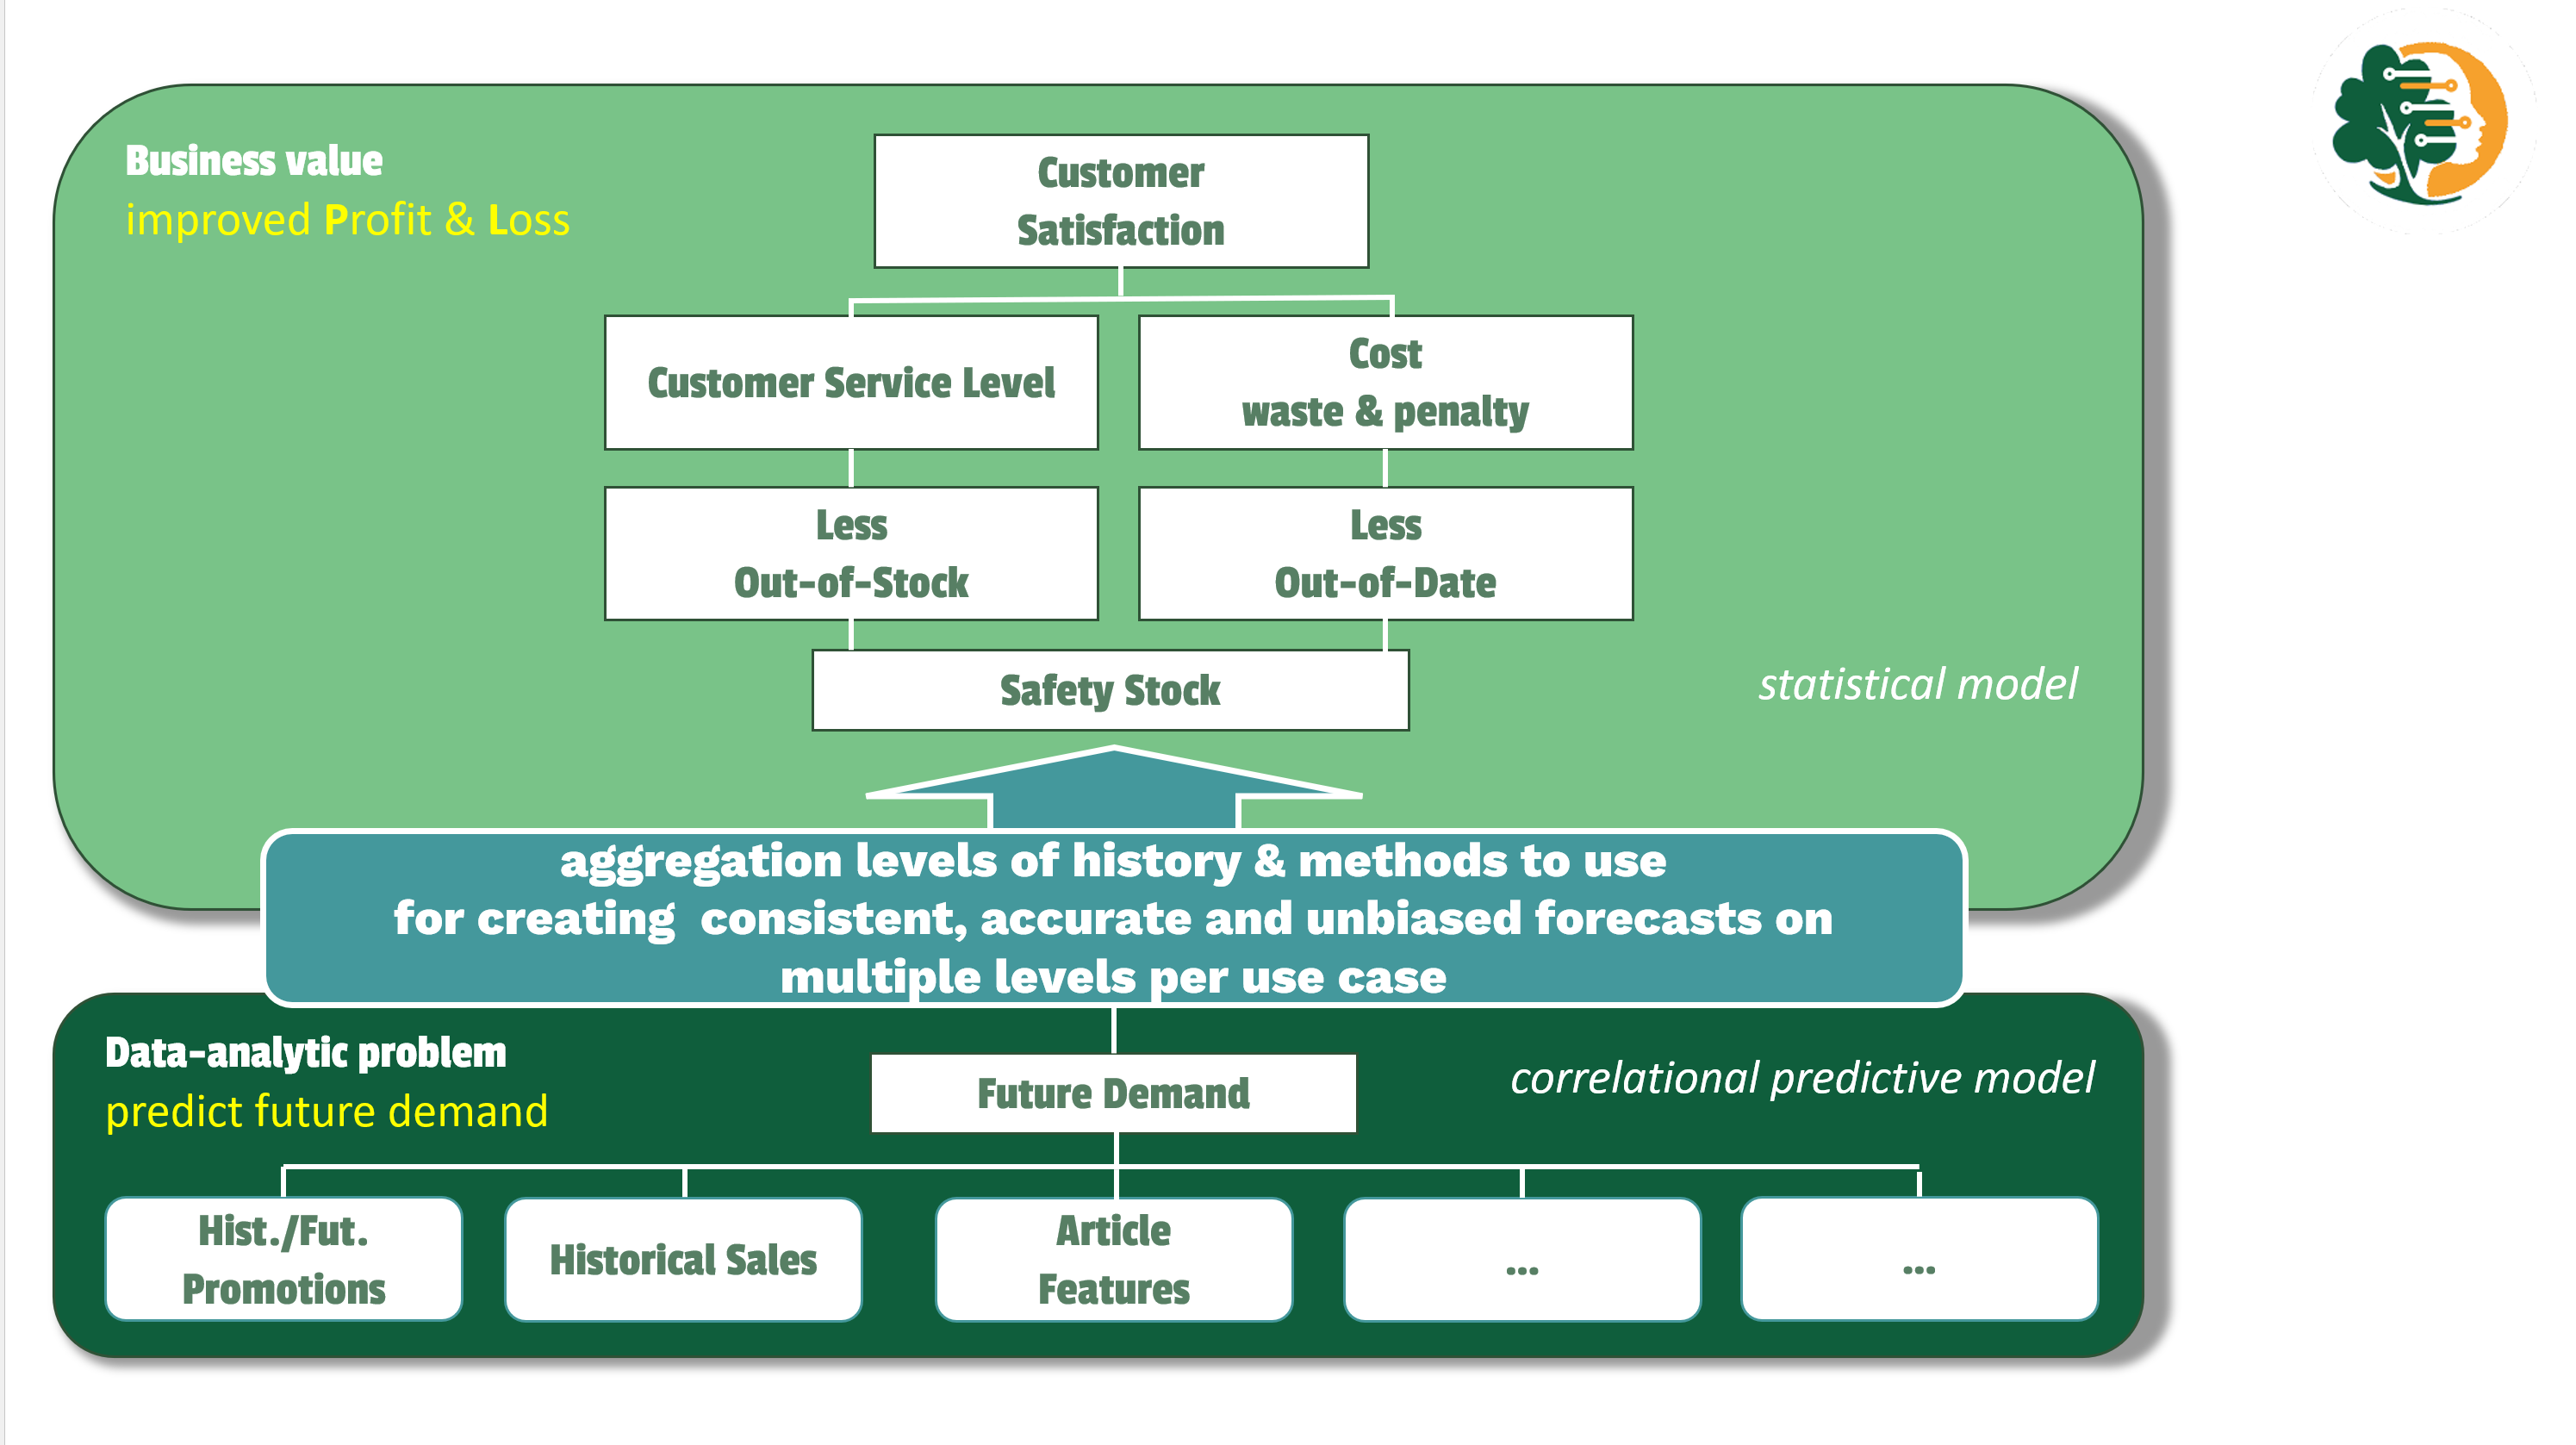
\includegraphics[width=1\linewidth,height=\textheight,keepaspectratio]{nb/../images/flowdown.png}

}

\end{figure}%

\chapter{References}\label{references}

\chapter*{References}\label{references-1}
\addcontentsline{toc}{chapter}{References}

\markboth{References}{References}

\phantomsection\label{refs}
\begin{CSLReferences}{1}{0}
\bibitem[\citeproctext]{ref-barrett_datatable_2024}
Barrett, T., Dowle, M., Srinivasan, A., Gorecki, J., Chirico, M.,
Hocking, T., Schwendinger, B., Stetsenko, P., Short, T., Lianoglou, S.,
Antonyan, E., Bonsch, M., Parsonage, H., Ritchie, S., Ren, K., Tan, X.,
Saporta, R., Seiskari, O., Dong, X., \ldots{} Krylov, I. (2024).
\emph{Data.table: {Extension} of 'data.frame'}.
\url{https://cran.r-project.org/web/packages/data.table/index.html}

\bibitem[\citeproctext]{ref-blokdyk_scor_2019}
BLOKDYK, G. (2019). \emph{{SCOR} {MODEL} {A} {COMPLETE} {GUIDE} - 2020
{EDITION}}. 5STARCOOKS.

\bibitem[\citeproctext]{ref-r_core_team_r_2024}
Core Team\}, \{R. (2024). \emph{R: {A} {Language} and {Environment} for
{Statistical} {Computing}}. R Foundation for Statistical Computing.
\url{https://www.R-project.org/}

\bibitem[\citeproctext]{ref-costa_crisp-ml_2022}
Costa, R. (2022). \emph{The {CRISP}-{ML} {Methodology}: {A}
{Step}-by-{Step} {Approach} to {Real}-{World} {Machine} {Learning}
{Projects}}. Independently published.

\bibitem[\citeproctext]{ref-debruine_glossary_2023}
DeBruine, L. (2023). \emph{Glossary: {Glossaries} for {Markdown} and
{Quarto} {Documents}}.
\url{https://cran.r-project.org/web/packages/glossary/}

\bibitem[\citeproctext]{ref-guja_generative_2025}
Guja, A., \& Siwiak, M. (2025). \emph{Generative {AI} for {Data}
{Analytics}.} Manning Publications Co. LLC 2025.

\bibitem[\citeproctext]{ref-hartshorn_machine_2017}
Hartshorn, S. (2017). \emph{Machine {Learning} {With} {Boosting}: {A}
{Beginner}'s {Guide}}.

\bibitem[\citeproctext]{ref-hyndmanaut2024}
Hyndman {[}aut, R., cre, cph, Athanasopoulos, G., Bergmeir, C., Caceres,
G., Chhay, L., Kuroptev, K., O'Hara-Wild, M., Petropoulos, F., Razbash,
S., Wang, E., Yasmeen, F., Garza, F., Girolimetto, D., Ihaka, R., R Core
Team, Reid, D., Shaub, D., \ldots{} Zhou, Z. (2024). \emph{Forecast:
Forecasting functions for time series and linear models}.
\url{https://cran.r-project.org/web/packages/forecast/index.html}

\bibitem[\citeproctext]{ref-hyndman__aut_fpp3_2024}
Hyndman {[}aut, R., cre, cph, Athanasopoulos, G., O'Hara-Wild, M.,
Palihawadana, N., Wickramasuriya, S., \& RStudio. (2024). \emph{fpp3:
{Data} for "{Forecasting}: {Principles} and {Practice}" (3rd
{Edition})}.
\url{https://cran.r-project.org/web/packages/fpp3/index.html}

\bibitem[\citeproctext]{ref-hyndman_forecasting_2021}
Hyndman, R. J., \& Athanasopoulos, G. (2021). \emph{Forecasting:
{Principles} and {Practice} (3rd ed)}. \url{https://otexts.com/fpp3/}

\bibitem[\citeproctext]{ref-kunapuli_ensemble_2023}
Kunapuli, G. (2023). \emph{Ensemble methods for machine learning}.
Manning.

\bibitem[\citeproctext]{ref-manokhin_practical_2023}
Manokhin, V. (2023). \emph{Practical guide to applied conformal
prediction in {Python}: Learn and apply the best uncertainty frameworks
to your industry applications}. {\textless{}}packt{\textgreater{}}.

\bibitem[\citeproctext]{ref-matthes_python_2019}
Matthes, E. (2019b). \emph{Python crash course: A hands-on,
project-based introduction to programming} (2nd edition). No Starch
Press.

\bibitem[\citeproctext]{ref-matthes2019}
Matthes, E. (2019a). \emph{Python crash course: A hands-on,
project-based introduction to programming} (2nd edition). No Starch
Press.

\bibitem[\citeproctext]{ref-molnar_introduction_2023}
Molnar, C. (2023). \emph{Introduction to conformal prediction with
{Python}: A short guide for quantifying uncertainty of machine learning
models} (First edition). Chistoph Molnar c/o MUCBOOK, Heidi Seibold.
\url{https://christophmolnar.com/books/conformal-prediction/}

\bibitem[\citeproctext]{ref-nixtlaux2fh}
\emph{Nixtla/hierarchicalforecast: Probabilistic hierarchical
forecasting 👑 with statistical and econometric methods.} (n.d.).
\url{https://github.com/Nixtla/hierarchicalforecast}

\bibitem[\citeproctext]{ref-nixtlaux2fm2024}
\emph{Nixtla/mlforecast}. (2024). Nixtla.
\url{https://github.com/Nixtla/mlforecast}

\bibitem[\citeproctext]{ref-nixtlaux2fs2024}
\emph{Nixtla/statsforecast}. (2024). Nixtla.
\url{https://github.com/Nixtla/statsforecast}

\bibitem[\citeproctext]{ref-nixtlaux2ft2024}
\emph{Nixtla/tsfeatures}. (2024). Nixtla.
\url{https://github.com/Nixtla/tsfeatures}

\bibitem[\citeproctext]{ref-ohara-wild2024a}
O'Hara-Wild, M., Hyndman, R., Wang, E., Cook, D., features), T. T.
(Correlation., \& method), L. C. (Guerrero's. (2024). \emph{Feasts:
Feature extraction and statistics for time series}.
\url{https://cran.r-project.org/web/packages/feasts/index.html}

\bibitem[\citeproctext]{ref-ohara-wild2024}
O'Hara-Wild, M., Hyndman, R., Wang, E., implementation), G. C. (NNETAR.,
Bergmeir, C., Hensel, T.-G., \& Hyndman, T. (2024). \emph{Fable:
Forecasting models for tidy time series}.
\url{https://cran.r-project.org/web/packages/fable/index.html}

\bibitem[\citeproctext]{ref-osullivan_introduction_2023}
O'Sullivan, C. (2023). Introduction to {SHAP} with {Python}. In
\emph{Introduction to SHAP with Python}.
\url{https://towardsdatascience.com/introduction-to-shap-with-python-d27edc23c454}

\bibitem[\citeproctext]{ref-osullivan_shap_2024}
O'Sullivan, C. (2024). {SHAP} with {Python} {[}Course{]}. In \emph{SHAP
with Python}. \url{https://adataodyssey.com/course/}

\bibitem[\citeproctext]{ref-porter_learn_2024}
Porter, L., \& Zingaro, D. (2024). \emph{Learn {AI}-assisted {Python}
programming: With {GitHub} {Copilot} and {ChatGPT}}. Manning.

\bibitem[\citeproctext]{ref-silver_inventory_2021}
Silver, E. A., Pyke, D. F., \& Thomas, D. J. (2021). \emph{Inventory and
production management in supply chains} (Fourth edition, first issued in
paperback). CRC Press, Taylor \& Francis Group.

\bibitem[\citeproctext]{ref-vandeput_inventory_2020}
Vandeput, N. (2020). \emph{Inventory optimization: Models and
simulations}. De Gruyter.

\bibitem[\citeproctext]{ref-vandeput_data_2021}
Vandeput, N. (2021). \emph{Data science for supply chain forecasting}
(Second edition). De Gruyter.

\bibitem[\citeproctext]{ref-vandeput_demand_2023}
Vandeput, N. (2023). \emph{Demand forecasting best practices}. Manning
Publications Co.

\bibitem[\citeproctext]{ref-wickham}
Wickham, H. (n.d.). \emph{R for data science (2e)}.
\url{https://r4ds.hadley.nz/}

\bibitem[\citeproctext]{ref-wickham_ggplot2_2024}
Wickham, H., Chang, W., Henry, L., Pedersen, T. L., Takahashi, K.,
Wilke, C., Woo, K., Yutani, H., Dunnington, D., Brand, T. van den,
Posit, \& PBC. (2024). \emph{ggplot2: {Create} {Elegant} {Data}
{Visualisations} {Using} the {Grammar} of {Graphics}}.
\url{https://cran.r-project.org/web/packages/ggplot2/index.html}

\end{CSLReferences}

\chapter{Resources}\label{resources}

\chapter{Resources}\label{sec-19-resources}

\begin{itemize}
\tightlist
\item
  \href{../notebooks/01_business_understanding.qmd}{Download the
  Business Understanding notebook (QMD) 💾}
\item
  \href{../notebooks/02_data_understanding.qmd}{Download the Data
  Understanding notebook (QMD) 💾}
\item
  \href{../pptx/PAF+s03.pptx}{Download EAISI Graduation Presentation
  (PPTX) 💾}
\item
  \href{notebooks.zip}{Download all notebooks (ZIP) 💾}
\end{itemize}


\backmatter


\end{document}
